%%%%%%%%%%%%%%%%%%%%%%%%%%%%%%%%%%%%%%%%%%%%%
%
% 2019main.tex (ICRR annual report 2019)
%
% Compiled using TexShop 4.44 on MAC OS 10.14.6
%
%%%%%%%%%%%%%%%%%%%%%%%%%%%%%%%%%%%%%%%%%%%%%
%
% main_header.tex
%
%\documentclass[twocolumn]{report} %MM
\documentclass[twocolumn,dvipdfmx]{report} %TS
\usepackage{multicol}

\makeatletter
\newenvironment{tablehere}
  {\def\@captype{table}}
  {}

\newenvironment{figurehere}
  {\def\@captype{figure}}
  {}
\makeatother

%\usepackage[dvips]{graphicx}
%\usepackage[dvipdfmx]{graphicx} %Sako 20180725
\usepackage{graphicx} % Sako comment out
\usepackage{amsmath,amssymb} %YT
\usepackage{times,mathptmx} %YT
\usepackage{url} %TY
\usepackage{subfig} %TY
%\usepackage{./stfloats} %TY11
\usepackage{AnRep}% 
\usepackage{color}
%\usepackage{footnote}
%\makesavenoteenv{table}
\usepackage{threeparttable}
\usepackage{epstopdf}
\usepackage{comment}
\usepackage{seqsplit}
\usepackage{supertabular}

\textwidth 42pc
\textheight 59pc  %%chnged !
\columnsep 1pc
\raggedbottom
\oddsidemargin -2.5pc
\evensidemargin -2.5pc
\topmargin -3pc  %%chnged !
\headsep .8pc
%\mathindent 1pc
\pagestyle{myheadings}

\def\textfraction{0.1} %TY10
\def\floatpagefraction{0.9} %TY10
\def\dblfloatpagefraction{0.9} %TY10

\def\nue{\nu_e}
\def\neb{\bar \nu_e}
\def\num{\nu_\mu}
\def\nmb{\bar \nu_\mu}
\def\nut{\nu_\tau}
\def\ntb{\bar \nu_\tau}
\def\nub{\bar \nu}
\def\dms{\Delta m^2}
\def\sst{\sin^2 2\theta}
\def\tasq{\tan^2\theta}
\def\sisq{\sin^2\theta}

%%% these are bitmap fonts
%%% use PostScript fonts instead these (03/28/2005 Y.Takeuchi)
%\newfont{\sff}{cmssi9} % for affiliation and section italic
%\newfont{\bigsf}{cmss12 scaled 2000} % for title
%\newfont{\midsf}{cmss12 scaled 1000} % for title's subscription
%\newfont{\bfsf}{cmssbx10 scaled 1200} % for title's subscription
%\newfont{\bfsfn}{cmssbx10 scaled 1000} % for title's subscription
%\newfont{\smlsf}{cmss12 scaled 600}  
                       % for section's subscription e.g.$_{\mbox{\smlsf 2}}$
%\newfont{\bigsff}{cmssi12 scaled 2000} % for title's italic

\newfont{\bigsf}{phvr8r scaled 2000} % for title (YT)
\newfont{\bfsf}{phvb8r scaled 1200}  % for title's subscription (YT)


\newcommand{\pmonth}{}
\newcommand{\spec}{}
\newcommand{\no}{}
\newcommand{\bi}{\bfseries\itshape}
\providecommand{\yen}{Y\llap=}

\newcommand{\lsim}{\mbox{\raisebox{-1.ex}
{$\stackrel{\textstyle <}{\textstyle \sim}$}}}
\newcommand{\gsim}{\mbox{\raisebox{-1.ex}
{$\stackrel{\textstyle >}{\textstyle \sim}$}}}
%\newcommand{\sstt}      {\sin^2 2\theta}
%\newcommand{\dms}       {\Delta m^2}
\newcommand{\plumin}[2]{^{+#1}_{-#2}}

\def\nue{\nu_e}
\def\neb{\bar \nu_e}
\def\num{\nu_\mu}
\def\nmb{\bar \nu_\mu}
\def\nut{\nu_\tau}
\def\ntb{\bar \nu_\tau}
\def\nub{\bar \nu}
\def\dms{\Delta m^2}
\def\sst{\sin^2 2\theta}
\def\tasq{\tan^2\theta}

%%%% these are bitmap fonts
%%%% use PS fonts, instead
%\font\lg=cmr12
%\font\bg=cmr17
%\font\sm=cmr7
%\font\fontA=cmr10 scaled \magstep3
%%\font\ssm=cmss12
%\newfont{\ssm}{cmssbx10 scaled 1200} % for title's subscription
%\font\tsmb=cmssbx10 %MM
%\font\ssml=cmss12   %MM
%\font\tsm=cmss10
%\font\utsm=cmss10
%\parindent=10pt

\def\utsm{\sf} %YT
\font\tsmb=phvb8r  %YT
\newfont{\ssm}{phvr8r scaled 1200} %YT
\def\tsm{\sf}  %YT

\def\overset#1\to#2{\mathop{#2}\limits^{#1}}
\def\underset#1\to#2{\mathop{#2}\limits_{#1}}
%\settabs 2 \columns
% A useful Journal macro
\def\Journal#1#2#3#4{{#1} {\bf #2}, #3 (#4)}

% Some useful journal names
\def\NCA{\em Nuovo Cimento}
\def\NIM{\em Nucl. Instrum. Methods}
\def\NIMA{{\em Nucl. Instrum. Methods} A}
\def\NPB{{\em Nucl. Phys.} B}
\def\PLB{{\em Phys. Lett.}  B}
\def\PRL{\em Phys. Rev. Lett.}
\def\PRD{{\em Phys. Rev.} D}
\def\ZPC{{\em Z. Phys.} C}
\def\APJ{\em Ap. J.}
\def\AP{\em Astroparticle Phys.}
\def\JPG{\em J. Phys. G: Nucl. Part. Phys.}

% Some other macros used in the sample text
\def\st{\scriptstyle}
\def\sst{\scriptscriptstyle}
\def\mco{\multicolumn}
\def\epp{\epsilon^{\prime}}
\def\vep{\varepsilon}
\def\ra{\rightarrow}
\def\ppg{\pi^+\pi^-\gamma}
\def\vp{{\bf p}}
\def\ko{K^0}
\def\kb{\bar{K^0}}
\def\al{\alpha}
\def\ab{\bar{\alpha}}
\def\be{\begin{equation}}
\def\ee{\end{equation}}
\def\bea{\begin{eqnarray}}
\def\eea{\end{eqnarray}}
\def\CPbar{\hbox{{\rm CP}\hskip-1.80em{/}}}%temp replacement due to no font

% Extracted from AASTeX (TY)
\newcommand\fdg{\mbox{$.\!\!^\circ$}}%

\renewcommand{\bibname}{AAA}%


\begin{document}
\sloppy   % 2018/7/31 TS

%%%%%%%%%%%%%%%%%%%%%%%%%%
% front and back pages (to be removed as last)
%%%%%%%%%%%%%%%%%%%%%% %%%%
%\begin{figure}[h]
%\begin{center}
%\includegraphics[width=24cm, angle=-90]{AnnualReport_cover.pdf}
%\caption{This is to show the front and back cover pages.  Real contents start from the next page.}
%\end{center}
%\end{figure}
%clearpage

%%%%%%%%%%%%%%%%%%%%%%
% modify here (start)
%%%%%%%%%%%%%%%%%%%%%%
%\input{preface/preface.tex} 
%%\input{preface/preface_simple.tex} 
%\setcounter{figure}{0}
%\setcounter{table}{0}
%\setcounter{page}{1}
%
%%\label{div}
%\input{division-contents.tex}

%\begin{comment}
  %%\label{nu}
%  \setcounter{figure}{0}
%  \setcounter{table}{0}
%  \input{neudiv/overview-neutrino.tex}
%  \input{neudiv/sk/sk.tex}
%  \input{neudiv/sk/t2k/t2k.tex}
%  \input{neudiv/xmass/xmass.tex}
%  \input{neudiv/hk/hk.tex}
%\end{comment}

%\begin{comment}
  %%\label{hecr}
%  \setcounter{figure}{0}
%  \setcounter{table}{0}
%  \input{hecrdiv/overview-hecr.tex}
%  \input{hecrdiv/gamma/gamma2019.tex}
%  \input{hecrdiv/TA/project-TA.tex}
%  \input{hecrdiv/Tibet/tibet.tex}
%  \input{hecrdiv/ALPACA/alpaca.tex}
%  \input{hecrdiv/hea/annualreport_HEA2018.tex}
%  \input{hecrdiv/others/others.tex}
%\end{comment}

%\begin{comment}
  %%\label{astro}
  %\color{red}
  \setcounter{figure}{0}
  \setcounter{table}{0}
  \twocolumn[
\begin{center}
\vspace{1pc} 
{\bigsf  ASTROPHYSICS AND GRAVITY DIVISION}
\label{astro}
\vspace{20pt}
\end{center}]

%%%%%%%%%%%%%%%%%%%%%%%%%%%%%%%%%%%%%%%%%%%%%%%%%%%%%%%%%%%%%%%%%%%%%%%%%%%%%%
% overview
%%%%%%%%%%%%%%%%%%%%%%%%%%%%%%%%%%%%%%%%%%%%%%%%%%%%%%%%%%%%%%%%%%%%%%%%%%%%%%
\section*{\sf Overview}
\vspace{3pt}
Astrophysics and Gravity Division consists of Gravitational Wave Group, 
The Observational Cosmology Group, Primary Cosmic Ray Group and Theory Group.

The Gravitational Wave Group conducts experimental research of gravitational wave with researchers of gravitational wave experiment and theory in Japan. The main items are the construction of the large scale cryogenic interferometer(KAGRA) at Kamioka underground and the operation of CLIO. For this purpose, KAGRA observatory was established at the beginning of the fiscal year of 2016 to assist the construction of KAGRA gravitational wave telescope. 

%Gravitational Wave Project Office (GWPO) was established at the beginning of the fiscal year of 2011 to assist the construction of KAGRA gravitational wave telescope. The main office is located at Kamioka since 2014. 

The Observational Cosmology Group studies the cosmic history based on deep multi-wavelength observations in collaboration with worldwide researchers. This group has started a new optical deep survey project with the wide-field imager of Hyper Suprime-Cam mounted on the Subaru telescope.

Theory Group conducts both theoretical study of the Universe and astroparticle physics.
\vspace{25pt}
 
  %!TEX root = ../../2019main.tex
%%%%%%%%%%%%%%%%%
% header 
%%%%%%%%%%%%%%%%%
\hrule
\section*{\bfsf  Gravitational Wave Group}
\vspace{12pt}
\hrule

% \input{astrodiv/gw/gwpo2014.tex}
\vspace{10pt}
\subsection*{\bi KAGRA Project Status}
\vspace{3pt}
\noindent {\sf [Spokesperson :\ Takashi UCHIYAMA]}

\vspace{3pt}
\noindent {\sf \small ICRR, The Univ.\ of Tokyo, Hida, Gifu 506-1205}

\subsubsection*{\bf Overview}
KAGRA, Large-scale Cryogenic Gravitational wave Telescope, aims at detecting gravitational waves and developing gravitational wave astronomy, which was established by the first detection of gravitational waves by LIGO. KAGRA employs a 3\,km L-shaped laser interferometer with a cryogenic mirror system placed underground at Kamioka\cite{kagra_review}. The KAGRA development is divided into two stages: the initial KAGRA (iKAGRA) and baseline KAGRA (bKAGRA). The iKAGRA interferometer is a simple Michelson interferometer with a 2-Watt laser, room-temperature mirrors, and a simple vibration isolation system. We completed the iKAGRA interferometer with a test run in April 2016\cite{ikagra_paper}. Then we proceeded to bKAGRA. 






Figure~\ref{fig:config} and \ref{fig:vis} show a schematic view of optical layout of the bKAGRA interferometer and the KAGRA vibration isolation systems. Table \ref{table:design_para} shows design parameter of the bKAGRA interferometer\cite{phase1_paper}. The bKAGRA interferometer will employ a Resonant Sideband Extraction (RSE) interferometer with 180-Watt laser, cryogenic Sapphire mirrors, and several kinds of vibration isolation systems. The bKAGRA interferometer should attain the sensitivity high enough for the detection of gravitational waves with the help of the high power laser and RSE interferometer to reduce the quantum noise, the cryogenic Sapphire mirrors to reduce the thermal noise, and the vibration isolation systems to reduce the seismic noise. Figure~\ref{fig:kagra-sensitivity} shows designed sensitivities of bKAGRA in case of Broadband RSE (BRSE) and of Detuned RSE (DRSE), where incoherent sum of the fundamental noise sources is assumed. Observation range for an in-spiral and merger of neutron-star binary reaches 135\,Mpc in BRSE and 153\,Mpc in DRSE with the same definition of the observation range as LIGO and Virgo. 


\begin{figure}
\begin{center}
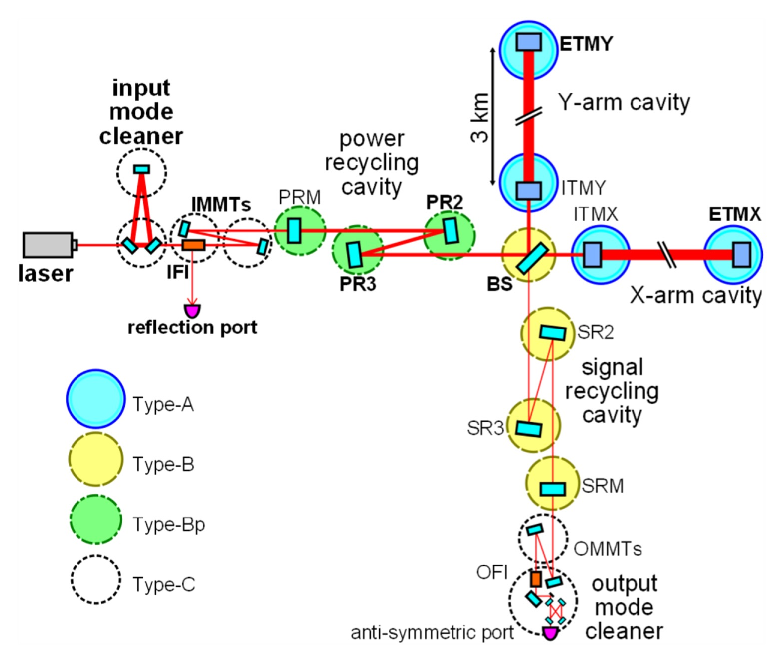
\includegraphics[width=8.5cm]{astrodiv/gw/overview/fig/kagra_config.eps}
\caption{Schematic view of the bKAGRA interferometer\cite{phase1_paper}. Type-A, Type-B, Type-Bp, and Type-C are the names of vibration isolation system for each mirror. }
\label{fig:config}
\end{center}
\end{figure}




\begin{figure}
\begin{center}
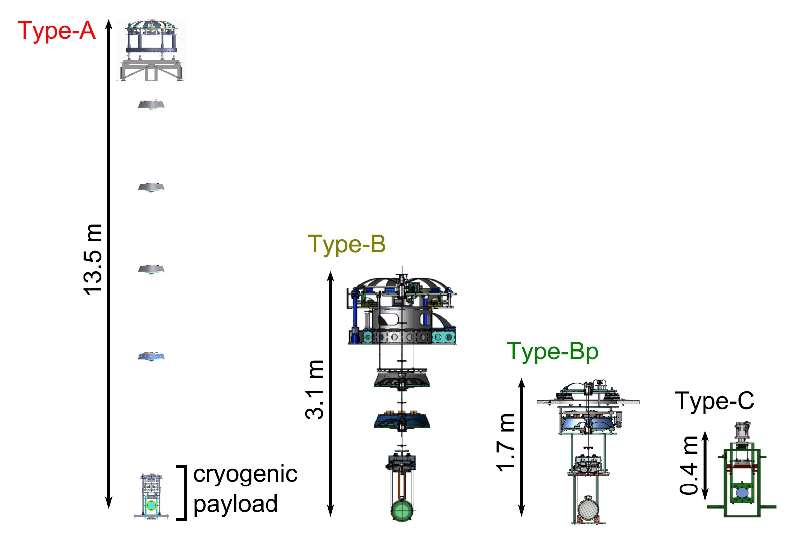
\includegraphics[width=8.5cm]{astrodiv/gw/overview/fig/suspensions.eps}
\caption{KAGRA vibration isolation systems\cite{phase1_paper}. KAGRA equips four kinds of vibration isolation systems such as Type-A, Type-B, Type-Bp, and Type-C.}
\label{fig:vis}
\end{center}
\end{figure}

\begin{table*} 
\begin{center} 
 \caption{\label{table:design_para}The design parameters of the bKAGRA interferometer\cite{phase1_paper}.}
 \begin{tabular}{llll}
  \hline
 Arm cavity length & 3000\,m & Test mass size & $\phi 22\,\mathrm{cm} \times 15\,\mathrm{cm}$ \\
Laser wave length & 1064\,nm & Mass of test mass & 22.8\,kg \\
Input power at PRM & 67W & Temperature of test mass & 22\,K \\
Arm intra-cavity power & 340\,kW & Beam radius at test mass & 3.5\,cm\\ 
ITM transmittance & 0.4\,\% & PRC/SRC lengths & 66.6\,m\\ 
PRM transmittance & 10\,\% & Detuning angle & 3.5\,deg\\  
SRM transmittance & 15\,\% & Homodyne angle & 135.1\,deg\\  \hline
%\hline\hline
\end{tabular}
\end{center} 
 \end{table*}






\begin{figure}
\begin{center}
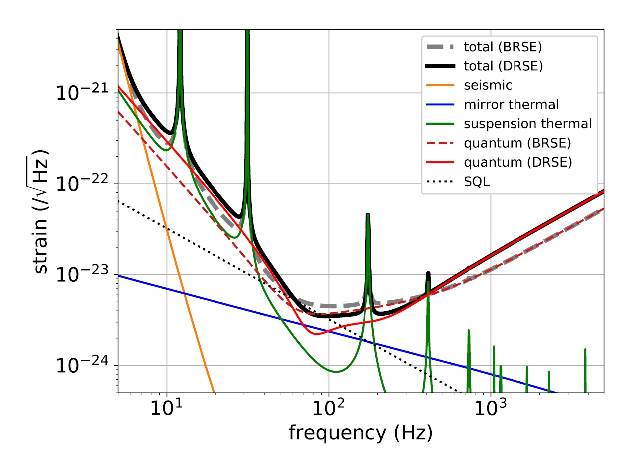
\includegraphics[width=8.5cm]{astrodiv/gw/overview/fig/kagra_sensitivity.eps}
\caption{The designed sensitivity of the bKAGRA interferometer\cite{phase1_paper}. "total", "seismic", "mirror thermal", "suspension thermal", "quantum", and "SQL" mean total sum of fundamental noise sources shown in this figure, seismic noise including gravity gradient noise, mirror thermal noise, suspension thermal noise, quantum noise, and standard quantum limit, respectively. The figure shows "total" and "quantum noise" in both Broadband RSE (BRSE) and Detuned RSE (DRSE) case. Observation range for an in-spiral and merger of neutron-star binary reaches 135\,Mpc in BRSE and 153\,Mpc in DRSE with the same definition of the observation range as LIGO and Virgo.}
\label{fig:kagra-sensitivity}
\end{center}
\end{figure}


Figure~\ref{fig:scenario} shows the international collaborative observation scenario\cite{scenario_paper}. LIGO conducted Observation 1 (O1) from September 12th, 2015 to January 19th, 2016 and Observation 2 (O2) from November 30th, 2016 to August 25th, 2017. Virgo joined O2 from August 1st, 2017. LIGO and Virgo started Observation  3 (O3) from April 1st, 2019 and O3 will continue by the end of April in 2020. KAGRA is aiming to join O3 in 2019.



\begin{figure}
\begin{center}
\includegraphics[width=8.5cm]{astrodiv/gw/overview/fig/scenario.eps}
\caption{International observation scenario\cite{scenario_paper}. Virgo was joined in Observation 2 (O2) from August 1st in 2017. LIGO and Virgo  started Observation 3 (O3) from April 1st in 2019. O3 will continue by the end of April in 2020. KAGRA is aiming to join O3 in 2019.}
\label{fig:scenario}
\end{center}
\end{figure}






In FY2018 we started with an operation of KAGRA interferometer as bKAGRA phase 1 which is 3\,km Michelson interferometer with two sapphire mirrors suspended by the Type-A vibration isolation systems. One sapphire mirror was cooled at 18\,K. The operation was done from April 28 to May 6 in 2018 and it was the first demonstration of operating km-class interferometer at cryogenic temperature. Figure~\ref{fig:dutyfactor} and Figure~\ref{fig:phase1_sens} shows a summary of daily status of the operation and a strain sensitivity comparing with noise sources\cite{phase1_paper}, respectively. Duty factor in the first half of the operation reached 88.6\%. The observation range for an in-spiral and merger of neutron-star binary and BH binary reached 17\,pc and 100\,pc, respectively. The longest continuous operation time was 11.1\,hour. 





\begin{figure}
\begin{center}
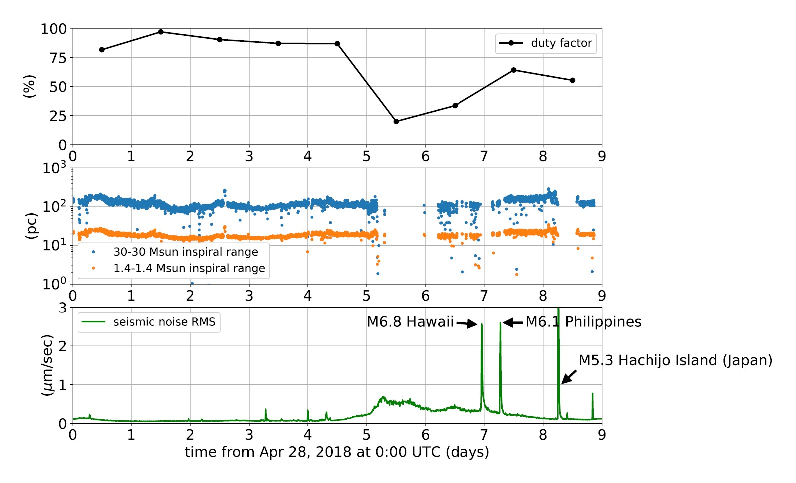
\includegraphics[width=8.5cm]{astrodiv/gw/overview/fig/dutyfactor.eps}
\caption{Daily status of bKAGRA phase 1 operation\cite{phase1_paper}. The figure shows daily duty factor (Top panel), inspiral range (Middle panel), and seismic noise level (Bottom panel) during the operation. The operation was done from April 28 to May 6 in 2018.}
\label{fig:dutyfactor}
\end{center}
\end{figure}





\begin{figure}
\begin{center}
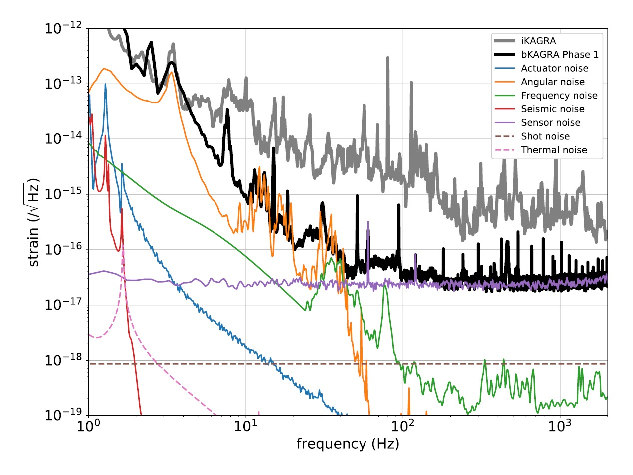
\includegraphics[width=8.5cm]{astrodiv/gw/overview/fig/phase1_sens.eps}
\caption{Strain sensitivity of KAGRA in phase 1 operation\cite{phase1_paper}. }
\label{fig:phase1_sens}
\end{center}
\end{figure}



After the bKAGRA phase 1 operation, we started construction of the bKAGRA interferometer with 40\,W laser power. What we have installed were an infrared laser system with the maximum power of 40\,W, two sets of arm length stabilization system using a green laser, calibration systems using photon radiation pressure, large beam baffles, transmission monitor systems, some optics consisting a signal recycling cavity and output optics, two input test masses called ITMX and ITMY in Figure~\ref{fig:config}, and so on. Physical Environmental Monitor (PEM) is a sensor network consisting several kinds of environmental sensors such as accelerometers, seismometers, magnetometers, thermometers, acoustic sound monitors, power monitors and so on. Purpose of PEM is to check the detector health, noise sources, and data quality in cooperation with the detector characterization group. We placed many sensors in the KAGRA site and monitoring has already started. 


We have tried lock acquisition of the X-arm cavity for the first time in parallel with the installation works mentioned above. The lock acquisition of the X-arm cavity was successfully achieved with helps of the arm length stabilization system. Then we carried out charcterization of the X-arm cavity. Table\ref{table:xarm} shows a summary of optical parameters of the X-arm cavity comparing with designed and measured values. 

\begin{table*} 
\begin{center} 
 \caption{\label{table:xarm}Optical parameters of the X-arm cavity\cite{xarm_com}.}
 \begin{tabular}{lll}
 Parameter name & Designed & Measured \\ \hline
 Cavity length & 3000\,m & 29999.990(2)\,m \\
 Finesse for 1064\,nm & 1530 & 1410(30) \\
Roundtrip loss for 1064\,nm & < 100\,ppm & 86(3)\,ppm \\
Finesse for 532\,nm & 49.2 & 41.0(3) \\ \hline 
\end{tabular}
\end{center} 
 \end{table*}

%There are progress reports in this annual report from Vacuum subgroup, Input Output Optics subgroup, Cryogenic subgroup, Digital control System subgroup, Analogue Electronics subgroup, Detector Characterization subgroup, ????, and Data analysis subgroup. 





%& Objects &Unit & Room temperature & Cryogenic  \\ \hline
%& Mirror temperature & K & $299$ & $17\, \textrm{and}\, 18$ \\  \hline
%$W _{\mathrm{front}}$ &Beam spot radius on front mirrors & mm & $4.9$ & $4.9$\\
%$W _{\mathrm{end}}$ &Beam spot radius on end mirrors & mm & $8.5$ & $8.5$\\ \hline
%& Material properties of Sapphire & & & \\ 
%$\alpha$ &Thermal expansion coefficient \cite{data_book, th_expansion_cryo} & 1/K& $5.4 \times 10^{-6}$ & $5.6 \times 10^{-9}$\\
%$\rho C$ &Specific heat per unit volume \cite{data_book} & J/K/m$^{3}$& $3.1 \times 10^{6}$ & $2.8 \times 10^{3}$\\
%$\kappa$ &Thermal conductivity \cite{data_book} & W/m/K& $46$ & $1.6 \times 10^{4}$\\
%$\sigma$ &Poisson's ratio\footnote{We found various values for the Poisson's ratio of sapphire between 0.23 and 0.30. We used the averaged value. 
%}& & $0.27$ & $0.27$\\
%$E$ &Young's modulus \cite{coating_Q}& Pa& $40 \times 10^{10}$ & $40\times 10^{10}$\\ 
%$\phi _{\mathrm{substr}}$ &Mechanical loss \cite{sapphire_subQ}& &  $1/4.6 \times 10^{6}$ & $1/1.5 \times 10^{8}$\\ \hline
%$\phi _{\mathrm{coat}}$ &Mechanical loss in coating films \cite{coating_Q} & & $4.0 \times 10^{-4}$ & $4.0 \times 10^{-4}$\\
%$d$ &Thickness of coating films & $\mathrm{\mu}$ m & $3.9$ & $3.9$\\
%



%In FY2017 we continued several installation and upgrade works toward the bKAGRA Phase 1. Fig. \ref{fig:bkagraphase1} and \ref{fig:vis} shows optical layout of bKAGRA Phase 1 and vibration isolation systems, respectively. We have installed mirrors of PRM, PR2, BS, ETMX, and ETMY in FY2017. ETMX is the sapphire mirror. ETMY is a spare sapphire mirror. PRM, PR2, and BS are made of fused silica. PRM, PR2 have been suspended Type-Bp vibration isolation systems. We have also upgraded the vibration isolation system for PR3 from Type-Bp' to Type-Bp. BS has been suspended by a Type-B vibration isolation system. ETMX and ETMY have been suspended Type-A vibration isolation systems. ETMY has been cooled 18\,K. All the optics needed for bKAGRA Phase 1 have been installed in FY2017 and we have successfully operated the cryogenic 3\,km Michelson interferometer from 28 April of 2018. 





%Here shows some photos about vibration isolation systems and mirrors installed in FY2017.





%\begin{figure}
%\begin{center}
%\includegraphics[width=8.5cm]{astrodiv/gw/overview/fig/bs.eps}
%\caption{Type-B vibration isolation system for beam splitter.}
%\label{fig:bs}
%\end{center}
%\end{figure}
%
%\begin{figure}
%\begin{center}
%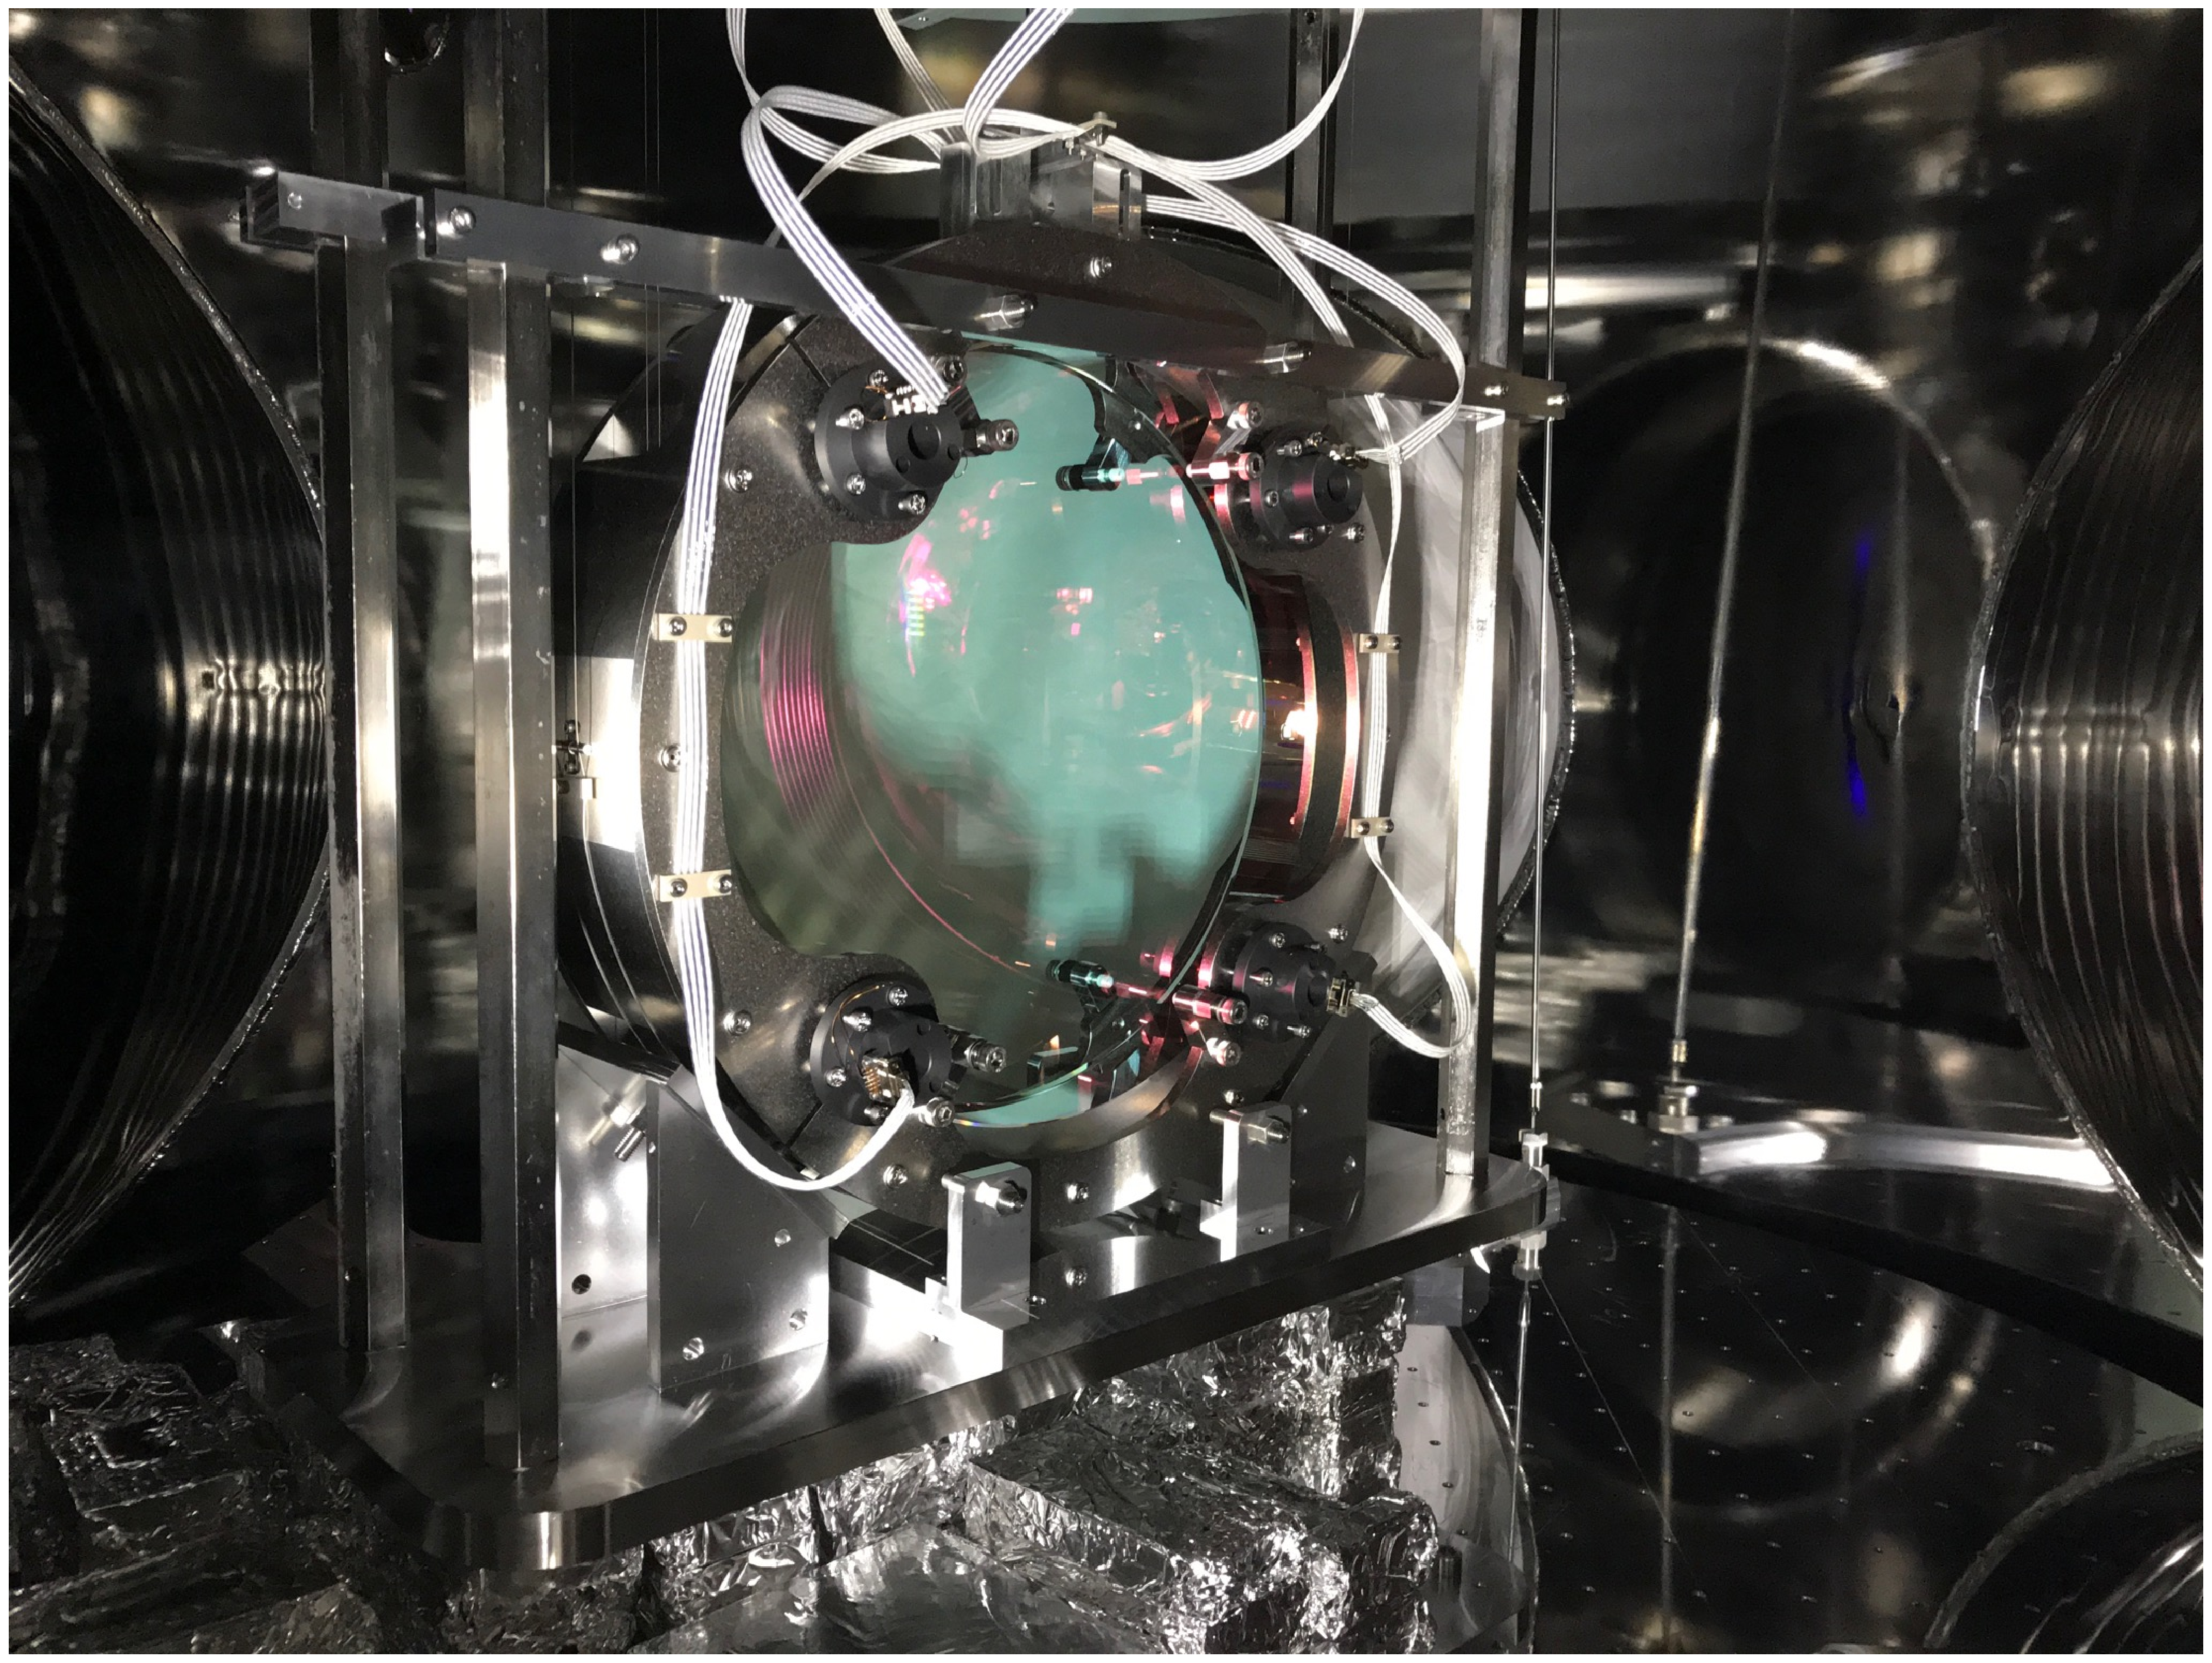
\includegraphics[width=8.5cm]{astrodiv/gw/overview/fig/bs2.eps}
%\caption{Beam splitter suspended in a vacuum chamber.}
%\label{fig:bs}
%\end{center}
%\end{figure}
%
%\begin{figure}
%\begin{center}
%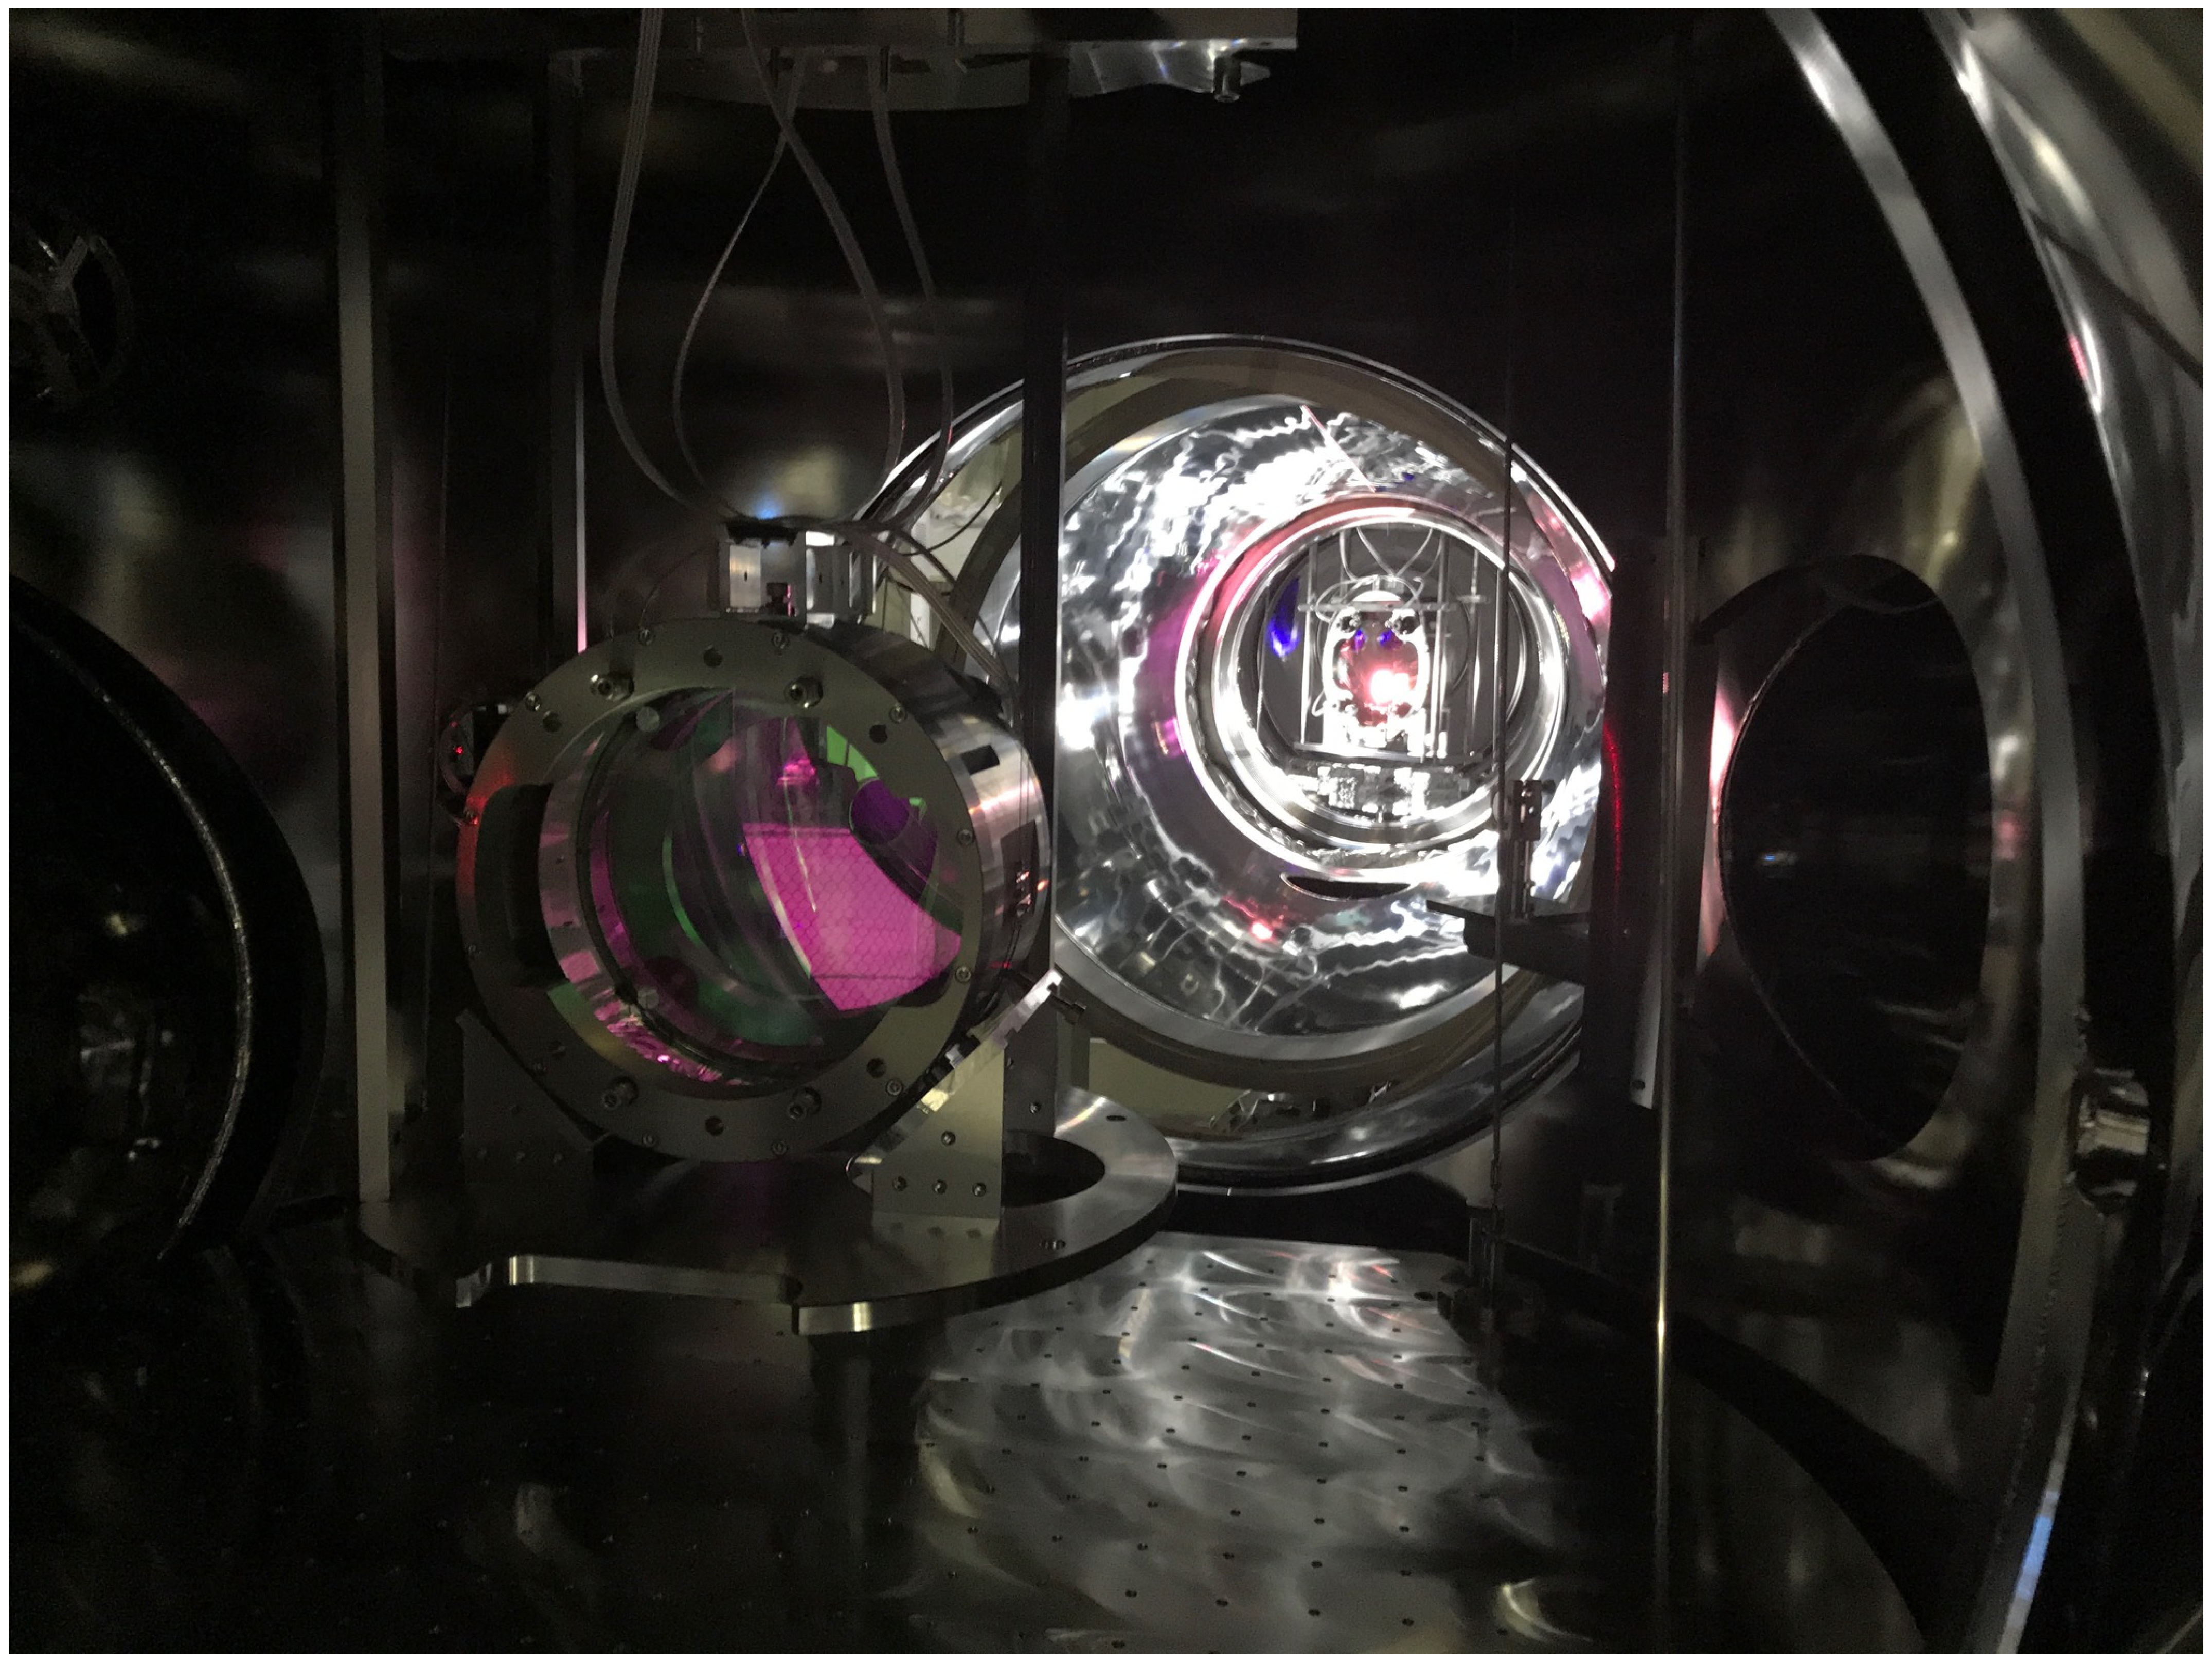
\includegraphics[width=8.5cm]{astrodiv/gw/overview/fig/pr2.eps}
%\caption{PR2 mirror suspended in a vacuum chamber. There is beam splitter behind the PR2 mirror.}
%\label{fig:bs}
%\end{center}
%\end{figure}
%
%    \begin{figure}
%\begin{center}
%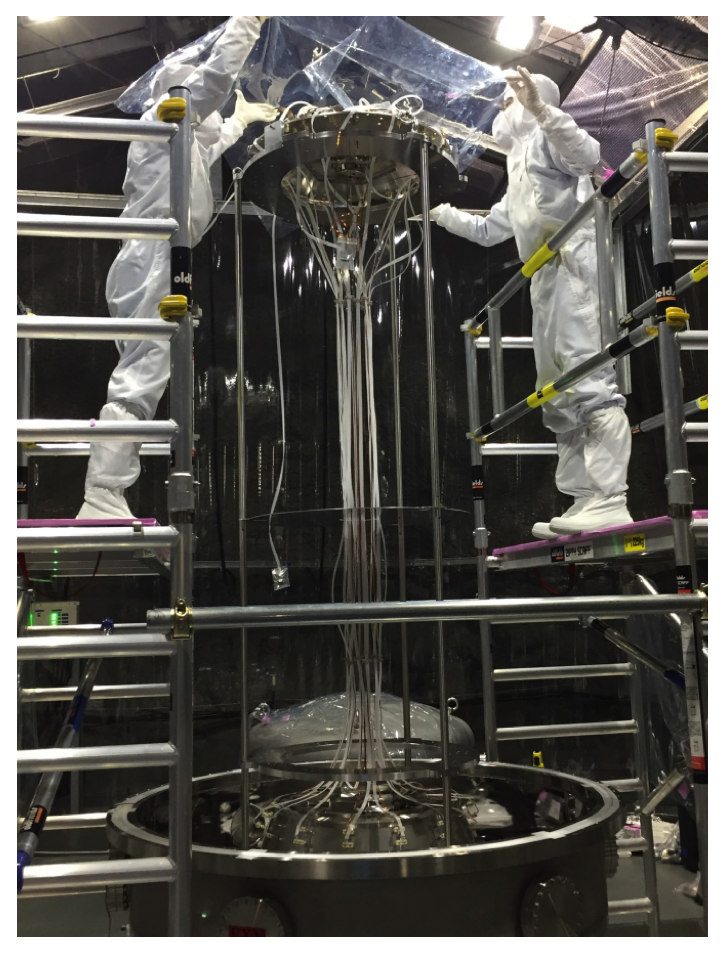
\includegraphics[width=8.5cm]{astrodiv/gw/overview/fig/typea.eps}
%\caption{A part of Type-A vibration isolation system.}
%\label{fig:bs}
%\end{center}
%\end{figure}



%In FY 2015 we installed many subsystems necessary for iKAGRA, including the connecting beam tubes, gate valves, input mode cleaner, input mode-matching telescope, power recycling folding mirrors, beam splitter, two end mirrors, suspension systems, other optics, optical levers, beam dumpers, analog electronics, digital control system, etc. Then we successfully locked the input mode cleaner, aligned the 3 km Michelson interferometer, and locked the interferometer.
%
%Then we performed a test run between Mar. 25 and Mar. 31, 2016. (The second test run was conducted in April 2016, but it will be reported in the annual report next year.) The input power to the beam splitter was 220 mW. The duty factor of the Michelson interferometer was 85.2 \%, and that of the input mode cleaner was 94.4 \%. The total lock time was 129.5 hours, and the longest lock was 3.6 hours. The typical strain sensitivity of the detector was $ 3\times 10^{-15} {\rm{Hz}}^{-1/2} $ at 100 Hz, which corresponds to a neutron star binary inspiral range of 0.77 pc.
%
%The interferometer was locked to the mid-fringe with a unity gain frequency of 8 Hz. All the suspended mirrors were controlled with the optical lever systems. The finesse and mode matching ratio of the pre-mode cleaner was 197 and 75 \%, respectively. The finesse and mode matching ratio of the input mode cleaner was 540 and 86.2 \%, respectively. The input mode cleaner mirrors, beam splitter, and end mirrors had Type-C suspension systems, while the power recycling folding mirror 3 had a Type-Bp' suspension system. The beam splitter, end mirrors, and power recycling folding mirror 3 were not in the vacuum because of insufficient commissioning time. The 80 Hz and 135 Hz monochromatic signals were applied to the control loop for the calibration of the interferometer. The interferometer lock was lost mainly because of the tidal drift of the mirrors. The noise spectrum was fluctuated by one order of magnitude. The sensitivity was limited mainly by intensity noise of laser light above 100 Hz.

%In the end of FY2015 we performed the first half of test run between Mar. 25 and Mar. 31, 2016. The details of the iKAGRA interferometer and the test run were described in the last annual report. In the beginning of FY 2016 we stopped the test run and improved the interferometer to reduce noise level and enhance stability. After the improvements, we performed the second half of test run from Apr. 11 to Apr. 25. Typical noise level at 100\,Hz was improved from $ 3\times 10^{-15} {\rm{Hz}}^{-1/2} $ to $ 7\times 10^{-16} {\rm{Hz}}^{-1/2} $ and an observation range of gravitational waves from binary coalescences of Neutron stars with 1.4 solar mass was extended from 0.77\,pc to 4.2\,pc. The duty cycle of the interferometer was increased from 85.2 \% to 90.4 \% even though Kumamoto earthquakes on Apr. 14 and 16 hit the test run. The longest lock of the interferometer reached 21.3 hours instead of 3.6 hours in the first half of the test run. 
%
%The scimon shift we took during the test run was the following. Each day was divided into three shift: 1:00 to 9:00, 9:00 to 17:00, and 17:00 to 1:00. In each shift slot one expert from ICRR, NAOJ, and KEK and two researchers from other universities/institutes were allocated. These scimons registered what happened as well as unusual events that they noticed during the shift. The scimon shift worked pretty smoothly. Finally, total of 65 people and cumulative total of 186 people from 35 institutes participated the shift works.
%
%All the data that was taken during the test run was stored and transferred to ICRR Kashiwa and Osaka City University in real time. The delayed mirroring of raw data was performed by Academia Sinica, Taiwan. KISTI, Korea was also copying the data. The transfer time from the KAGRA site to surface, ICRR Kashiwa, and Osaka City University was 0.3 sec, 2.5 sec, and 3 sec, respectively. The data management system worked very well.

%We started upgrading the interferometer from iKAGRA to bKAGRA after the test run, because we plan to operate the cryogenic 3\,km Michelson interferometer by the end of March 2018. The upgrading works are on going by many sub-groups. We give reports in the following sections from the vacuum sub-group, the input and output optics sub-group, the cryogenic sub-group, the digital control system sub-group, the detector characterization sub-group, and the mirror subgroup.


%The photos of  KAGRA taken in FY 2015 are shown (Fig.~\ref{fig:entrance} - Fig.~\ref{fig:PR3}).
%
%\begin{figure}
%\begin{center}
%\includegraphics[width=8.5cm]{astrodiv/gw/Overview/fig/entrance.eps}
%\caption{Entrance of the KAGRA tunnel.}
%\label{fig:entrance}
%\end{center}
%\end{figure}
%
%\begin{figure}
%\begin{center}
%\includegraphics[width=8.5cm]{astrodiv/gw/Overview/fig/chambers.eps}
%\caption{Vacuum chambers in the central area.}
%\label{fig:chambers}
%\end{center}
%\end{figure}
%
%\begin{figure}
%\begin{center}
%\includegraphics[width=8.5cm]{astrodiv/gw/Overview/fig/cryostat.eps}
%\caption{Cryostat for the cryogenic mirror and the shaft for the vibration isolation system.}
%\label{fig:cryostat}
%\end{center}
%\end{figure}
%
%\begin{figure}
%\begin{center}
%\includegraphics[width=8.5cm]{astrodiv/gw/Overview/fig/slope.eps}
%\caption{Slope to the 2nd floor.}
%\label{fig:slope}
%\end{center}
%\end{figure}
%
%\begin{figure}
%\begin{center}
%\includegraphics[width=8.5cm]{astrodiv/gw/Overview/fig/beamtube.eps}
%\caption{3-km beam tube in the Y-arm tunnel.}
%\label{fig:beamtube}
%\end{center}
%\end{figure}
%
%\begin{figure}
%\begin{center}
%\includegraphics[width=8.5cm]{astrodiv/gw/Overview/fig/PSL.eps}
%\caption{Pre-stabilized laser for iKAGRA.}
%\label{fig:PSL}
%\end{center}
%\end{figure}
%
%\begin{figure}
%\begin{center}
%\includegraphics[width=8.5cm]{astrodiv/gw/Overview/fig/MC.eps}
%\caption{Mirrors and suspension systems of the input mode cleaner.}
%\label{fig:MC}
%\end{center}
%\end{figure}
%
%\begin{figure}
%\begin{center}
%\includegraphics[width=8.5cm]{astrodiv/gw/Overview/fig/PR3.eps}
%\caption{Power recycling folding mirror and its suspension system.}
%\label{fig:PR3}
%\end{center}
%\end{figure}

We also enhanced the international collaborations with the Einstein Telescope (ET) project, LIGO, Virgo, Korean and other Asian groups mainly based on the JSPS core-to-core program.

The rapidly progressing status of KAGAR were presented in many international conferences. Many papers about the progress of KAGRA were also published \cite{kagra_review}, \cite{phase1_paper}, \cite{xarm_com}. We also presented activities on our web-page.\cite{KAGRA}

\begin{thebibliography}{99}


\bibitem{kagra_review} "KAGRA: 2.5 generation interferometric gravitational wave detector",
KAGRA collaboration, Nature Astronomy, Vol. 3, January 2019, 35-40

\bibitem{ikagra_paper} "Construction of KAGRA: an underground gravitational-wave observatory",
KAGRA collaboration,
Prog. Theor. Exp. Phys. 2018, 013F01 (2018)

\bibitem{scenario_paper} "Prospects for observing and localizing gravitational-wave transients with Advanced LIGO, Advanced Virgo and KAGRA",
Abbott, B.P., Abbott, R., Abbott, T.D. et al. arXiv:1304.0670v9 [gr-qc]






\bibitem{phase1_paper} "First cryogenic test operation of underground km-scale gravitational-wave observatory KAGRA",
KAGRA collaboration, Class. Quantum Grav. 36 165008 (2019)




\bibitem{xarm_com} "An arm length stabilization system for KAGRA and future gravitational-wave detectors",
KAGRA collaboration,
to be published in Class. Quantum Grav. (2019)



%
%\bibitem{michimura} "Mirror actuation design for the interferometer control of the KAGRA gravitational wave telescope",
%Yuta Michimura, Tomofumi Shimoda, Takahiro Miyamoto, Ayaka Shoda, Koki Okutomi, Yoshinori Fujii, Hiroki Tanaka, Mark A. Barton, Ryutaro Takahashi, Yoichi Aso, Tomotada Akutsu, Masaki Ando, Yutaro Enomoto, Raffaele Flaminio, Kazuhiro Hayama, Eiichi Hirose, Yuki Inoue, Takaaki Kajita, Masahiro Kamiizumi, Seiji Kawamura, Keiko Kokeyama, Kentaro Komori, Rahul Kumar, Osamu Miyakawa, Koji Nagano, Masayuki Nakano, Naoko Ohishi, Ching Pin Ooi, Fabian Erasmo Pena Arellano, Yoshio Saito, Katsuhiko Shimode, Kentaro Somiya, Hiroki Takeda, Takayuki Tomaru, Takashi Uchiyama, Takafumi Ushiba, Kazuhiro Yamamoto, Takaaki Yokozawa, Hirotaka Yuzurihara, Classical and Quantum Gravity 34, 225001(2017)
%
%\bibitem{gif} "Design and operation of a 1500-m laser strainmeter installed at underground site in Kamioka",
%Akito Araya, Akiteru Takamori, Wataru Morii, Kouseki Miyo, Masatake Ohashi, Kazuhiro Hayama, Takashi Uchiyama, Shinji Miyoki and Yoshio Saito, Earth, Planets and Space 69, 77 (2017)
%




\bibitem{KAGRA} http://gwcenter.icrr.u-tokyo.ac.jp/en/

\end{thebibliography}



%\cite{}



\vspace{10pt}
\subsubsection*{\bf Vacuum system for KAGRA}
\vspace{3pt}
\noindent {\sf [Spokesperson :\ Takashi UCHIYAMA]}

\vspace{3pt}
\noindent {\sf \small ICRR, The Univ.\ of Tokyo, Hida, Gifu 506-1205}

We firstly pumped six vacuum chambers those are IFI, IMM, PRM, PR3, PR2, and BS and vacuum pressure achieved order of $10^{-5}$\,Pa. We made control boxes for seven large gate valves those are GVmc between MCF and IFI, GVbsx between BS and IXC, GVitmx between IXA and the X-arm tube, GVetmx between the X-arm and EXA, GVbsy between BS and IYC, GVitmy between IYA and the Y-arm tube, and GVetmy between the Y-arm and EYA. The control boxes has open/close control buttons and indicators. The GVs will be controlled by remotely via KAGRA machine control system which has Programable Logic Circuits through the control boxes.

%The central part of the KAGRA interferometer 
%
%
%The vacuum sub-group of the KAGRA project has been designed and fabricated two vacuum chambers for BRT (Beam Reducing Telescope) in 2016. Both chambers have already placed at the both end experiment rooms. The BRT chamber is made of SUS304 and dimensions are diameter of 1200\,mm, height of 2400\,mm, and weight of 1990\,kg. 
%
%We procured 16 sets of Turbo Molecular Pumps (TMP), 17 sets of root pumps, and 10 sets of ion pumps. Evacuation speed of the TMPs, the root pumps, and the ion pumps are larger than 2000\,L/s for N$_{2}$ and H$_{2}$, 600\,L/s for N$_{2}$ and H$_{2}$, and 800\,L/s for N$_{2}$ and 1200\,L/s for H$_{2}$, respectively. Finally, KAGRA has 17 sets of TMP pumping units consisting of a TMP and a root pump and 10 sets of TMP and ION pumping units consisting of a TMP, a root pump, and an ion pump. We placed 15 sets of the TMP pumping units in the center experiment room, 1 set of the TMP pumping unit in the both end experiment rooms, and 5 sets of the TMP and ION pumping units in the both arm ducts.
%
%

\input{astrodiv/gw/ioo/ioo.tex}
\subsubsection*{\bf Cryogenic system}
\noindent {\sf [Spokesperson :\ Takafumi USHIBA]}

\noindent {\sf \small ICRR, The Univ.\ of Tokyo, Kashiwa, Chiba 277-8582}
\vspace{3pt}

A key feature of KAGRA is to cool four sapphire mirrors, which are used for constitution of two arm cavity, to 20\,K. Members working for a cryogenic system, which plays an important role for achieving this unique characteristics, is mainly constituted by that of ICRR, KEK, and the University of Toyama. Here, we summarize the activity of members of ICRR in FY 2017.

\paragraph*{\bi Cryogenic payload}

A KAGRA sapphire mirror is suspended by 9-stage suspension and its bottom 4 stages that include sapphire mirror is called cryogenic payload. The first cryogenic payload with a sapphire mirror was installed at Kamioka in November, 2017. Figure \ref{fig:KAGRAcryo payload} shows the cryogenic payload installed at KAGRA site. This payload was cooled down after installation and reached about 18\,K, which is below the target temperature of KAGRA, 20\,K.

Performance evaluation of sensors and actuators was performed at the site after cooling. It was then confirmed that all sensors and actuators on the cryogenic payload worked even at cryogenic temperature. Damping feedback system for the suspension eigenmode was also implemented, which is significant to operate KAGRA as an interferometer.

\begin{figure}[hbtp]
\begin{center}
\includegraphics[width=0.4\textwidth]{astrodiv/gw/cry/KAGRAcryo_payload.eps}
\caption{\utsm \noindent{\narrower{Cryogenic payload installed into the cryostat at KAGRA site}}}
\label{fig:KAGRAcryo payload}
\end{center}
\end{figure}

\paragraph*{\bi Pure aluminum heat conductor}

In order to cool the mirror down to 20\,K, it is necessary to utilize a high thermal-conductive heat conductor because at cryogenic temperature, especially below 100\,K, thermal radiation becomes small and cannot cool the mirror effectively. However, these heat conductors can easily induce vibration that worsens the KAGRA sensitivity. It is therefore important for the heat conductor to have flexibility enough to reduce the vibration transmission via itself. To realize high thermal conductivity and flexibility, Stranded cables made of pure aluminum of 99.9998\% (5N8 aluminum) are used for KAGRA heat conductor.

In FY 2017, thermal conductivity and flexibility measurement of the heat conductor were performed. Then, we measured a thermal conductivity of $1.85\times10^{4}$\,W/m/K at 10\,K, which is high sufficiently for applying to heat conductors for KAGRA. We also measured a spring constant of stranded heat conductor and compared with that of a single aluminum wire. Then, we confirmed that a spring constant of this stranded aluminum heat conductor is 43 times smaller than that of the single one.

\paragraph*{\bi Vibration measurement inside the cryostat}
We should use huge cryostat (roughly saying, diameter and hight are both 4\,m) in order to install the cryogenic payload and two-layer radiation shields. The resonant frequency of vibration modes of such huge structures is several tens of hertz, which covers KAGRA observation band. So, it is important to make a research for eigenmodes of the cryostat and implement their damping.

An interferometric accelerometer that can be fundamentally used even at the cryogenic temperature was developed. vibration level measurement inside the cryostat under the room temperature condition by using this accelerometer was performed. Then, we found that there is 1000 times lager vibration around 30\,Hz than typical ground vibration of KAGRA site. We also confirmed vibration from the cryocoolers are slightly larger than the ground vibration as well. 

\paragraph*{\bi Magnetic field measurement}

Coil magnet actuators are adopted to control the cryogenic payload, and sapphire mirror has a small magnet on its AR side. So, fluctuation of magnetic field around the payload make some force to the mirror and shake it. Magnetic field of the earth is small enough but there are many devices around the payload such as cryocoolers, vacuum pump, and so on. So, magnetic field generated by these devices should be well studied.

We compared the magnetic field when the cryocoolers are working with that when they are not working. As a result, we confirmed that there are several periodic magnetic field generated by the cryocoolers. Further investigation for these magnetic field issue is promoting.

\paragraph*{\bi Master theses}

Two Master thesis, {\it Vibration Analysis of Cryostat on KAGRA Site} and {\it A Study of the KAGRA Cryogenic Payload System and its Conduction Cooling}, were accepted in FY 2017. 

\paragraph*{\bi Acknowledgement}

Mechanical workshops of Institute for Solid State Physics (The University of Tokyo, Kashiwa campus) and Mechanical Engineering Center of KEK make a large contribution through providing many products for our research.
\vspace{10pt}
\subsubsection*{\bf Vibration Isolation System Type-A}
\vspace{3pt}
\noindent {\sf [Spokesperson :\ Lucia Trozzo ]}

\vspace{3pt}
\noindent {\sf \small ICRR, The Univ.\ of Tokyo, Hida, Gifu 506-1205}

\vspace{3pt}

Text here
%!TEX root = ../../../2019main.tex
\vspace{10pt}
\subsubsection*{\bf Vibration Isolation System Type-B}
\vspace{3pt}
\noindent {\sf [Spokesperson :\ Fabian Pe\~{n}a Arellano ]}

\vspace{3pt}
\noindent {\sf \small ICRR, The Univ.\ of Tokyo, Hida, Gifu 506-1205}

\vspace{3pt}


Besides the four Type-A suspensions KAGRA relies on smaller suspensions
for other mirrors which are always at room temperature. The Type-B
suspension is used for the beam splitter and the three signal recycling
mirrors, whereas the Type-Bp is used for the three power recycling
mirrors.

\begin{figure}[h]
\begin{centering}
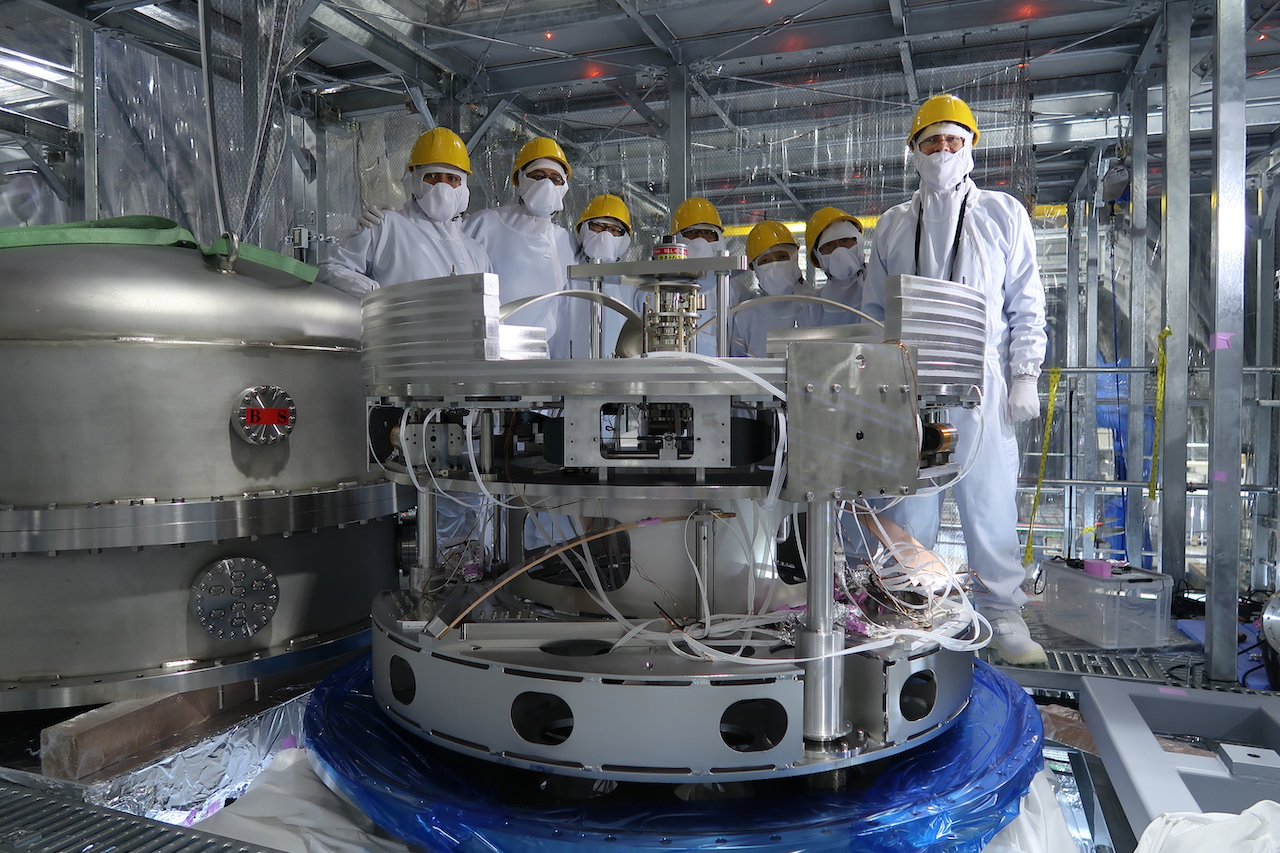
\includegraphics[width=0.48\textwidth, bb=0 0 1280 853]{astrodiv/gw/vis-b/typeB_team_01.jpg}
\par\end{centering}

\caption{The IP of the beam splitter in the vacuum chamber and the installation
team.}
\end{figure}


As in Type-A suspension, in Type-B suspension the first vibration
isolation stage is the Inverted Pendulum (IP), whose main goal is
to passively attenuate the persistent horizontal microseismic motion
produced by ocean activity. Typical resonant frequencies for these
IPs are between 60 mHz and 80 mHz in order attenuate the microseismic
peak at around 200 mHz. The following three stages, intended for vertical
isolation, are three geometric anti-spring filters. The first one
lies directly on top of the IP table while the other two hang from
it as the masses of a multi-stage pendulum. As in the case of the
IP, GAS filters are devices capable of supporting loads of hundreds
of kilograms and at the same time achieving resonant frequencies of
a few hundreds of millihertz. The horizontal position of the IP and
the vertical positions of the GAS filters are measured with Linear
Variable Differential Transformers (LVDTs) and are adjusted with coil-magnet
actuators which also damp the mechanical resonant motion. The typical
resolution of the LVDTs are below 0.2 $\mu$m. From the lowermost
GAS filter the payload hangs. The payload, which is common to Type-B
and Type-Bp suspensions, comprises the optic, its marionette and their
respective recoil masses. The recoil mass of the marionette holds
local displacement sensors to monitor six degrees of freedom and coil-magnet
actuators for damping the resonant modes of oscillation of the suspension
itself. The sensors have typical resolutions of about 20 nm. The recoil
mass of the mirror holds coil-magnet actuators only and the system
relies on an optical lever to monitor the tilt and position of the
optic from the ground.

The Type-Bp suspension is shorter and comprises two GAS filters and
the payload. The uppermost GAS filter lies directly on the ground
while the lowermost one has its own recoil mass in order to attenuate
motion which may be excited by the microseismic motion of the ground.
%!TEX root = ../../../2019main.tex
%%
% main_header.tex
%
%\documentclass[twocolumn]{report} %MM
\documentclass[twocolumn,dvipdfmx]{report} %TS
\usepackage{multicol}

\makeatletter
\newenvironment{tablehere}
  {\def\@captype{table}}
  {}

\newenvironment{figurehere}
  {\def\@captype{figure}}
  {}
\makeatother

%\usepackage[dvips]{graphicx}
%\usepackage[dvipdfmx]{graphicx} %Sako 20180725
\usepackage{graphicx} % Sako comment out
\usepackage{amsmath,amssymb} %YT
\usepackage{times,mathptmx} %YT
\usepackage{url} %TY
\usepackage{subfig} %TY
%\usepackage{./stfloats} %TY11
\usepackage{AnRep}% 
\usepackage{color}
%\usepackage{footnote}
%\makesavenoteenv{table}
\usepackage{threeparttable}
\usepackage{epstopdf}
\usepackage{comment}
\usepackage{seqsplit}
\usepackage{supertabular}

\textwidth 42pc
\textheight 59pc  %%chnged !
\columnsep 1pc
\raggedbottom
\oddsidemargin -2.5pc
\evensidemargin -2.5pc
\topmargin -3pc  %%chnged !
\headsep .8pc
%\mathindent 1pc
\pagestyle{myheadings}

\def\textfraction{0.1} %TY10
\def\floatpagefraction{0.9} %TY10
\def\dblfloatpagefraction{0.9} %TY10

\def\nue{\nu_e}
\def\neb{\bar \nu_e}
\def\num{\nu_\mu}
\def\nmb{\bar \nu_\mu}
\def\nut{\nu_\tau}
\def\ntb{\bar \nu_\tau}
\def\nub{\bar \nu}
\def\dms{\Delta m^2}
\def\sst{\sin^2 2\theta}
\def\tasq{\tan^2\theta}
\def\sisq{\sin^2\theta}

%%% these are bitmap fonts
%%% use PostScript fonts instead these (03/28/2005 Y.Takeuchi)
%\newfont{\sff}{cmssi9} % for affiliation and section italic
%\newfont{\bigsf}{cmss12 scaled 2000} % for title
%\newfont{\midsf}{cmss12 scaled 1000} % for title's subscription
%\newfont{\bfsf}{cmssbx10 scaled 1200} % for title's subscription
%\newfont{\bfsfn}{cmssbx10 scaled 1000} % for title's subscription
%\newfont{\smlsf}{cmss12 scaled 600}  
                       % for section's subscription e.g.$_{\mbox{\smlsf 2}}$
%\newfont{\bigsff}{cmssi12 scaled 2000} % for title's italic

\newfont{\bigsf}{phvr8r scaled 2000} % for title (YT)
\newfont{\bfsf}{phvb8r scaled 1200}  % for title's subscription (YT)


\newcommand{\pmonth}{}
\newcommand{\spec}{}
\newcommand{\no}{}
\newcommand{\bi}{\bfseries\itshape}
\providecommand{\yen}{Y\llap=}

\newcommand{\lsim}{\mbox{\raisebox{-1.ex}
{$\stackrel{\textstyle <}{\textstyle \sim}$}}}
\newcommand{\gsim}{\mbox{\raisebox{-1.ex}
{$\stackrel{\textstyle >}{\textstyle \sim}$}}}
%\newcommand{\sstt}      {\sin^2 2\theta}
%\newcommand{\dms}       {\Delta m^2}
\newcommand{\plumin}[2]{^{+#1}_{-#2}}

\def\nue{\nu_e}
\def\neb{\bar \nu_e}
\def\num{\nu_\mu}
\def\nmb{\bar \nu_\mu}
\def\nut{\nu_\tau}
\def\ntb{\bar \nu_\tau}
\def\nub{\bar \nu}
\def\dms{\Delta m^2}
\def\sst{\sin^2 2\theta}
\def\tasq{\tan^2\theta}

%%%% these are bitmap fonts
%%%% use PS fonts, instead
%\font\lg=cmr12
%\font\bg=cmr17
%\font\sm=cmr7
%\font\fontA=cmr10 scaled \magstep3
%%\font\ssm=cmss12
%\newfont{\ssm}{cmssbx10 scaled 1200} % for title's subscription
%\font\tsmb=cmssbx10 %MM
%\font\ssml=cmss12   %MM
%\font\tsm=cmss10
%\font\utsm=cmss10
%\parindent=10pt

\def\utsm{\sf} %YT
\font\tsmb=phvb8r  %YT
\newfont{\ssm}{phvr8r scaled 1200} %YT
\def\tsm{\sf}  %YT

\def\overset#1\to#2{\mathop{#2}\limits^{#1}}
\def\underset#1\to#2{\mathop{#2}\limits_{#1}}
%\settabs 2 \columns
% A useful Journal macro
\def\Journal#1#2#3#4{{#1} {\bf #2}, #3 (#4)}

% Some useful journal names
\def\NCA{\em Nuovo Cimento}
\def\NIM{\em Nucl. Instrum. Methods}
\def\NIMA{{\em Nucl. Instrum. Methods} A}
\def\NPB{{\em Nucl. Phys.} B}
\def\PLB{{\em Phys. Lett.}  B}
\def\PRL{\em Phys. Rev. Lett.}
\def\PRD{{\em Phys. Rev.} D}
\def\ZPC{{\em Z. Phys.} C}
\def\APJ{\em Ap. J.}
\def\AP{\em Astroparticle Phys.}
\def\JPG{\em J. Phys. G: Nucl. Part. Phys.}

% Some other macros used in the sample text
\def\st{\scriptstyle}
\def\sst{\scriptscriptstyle}
\def\mco{\multicolumn}
\def\epp{\epsilon^{\prime}}
\def\vep{\varepsilon}
\def\ra{\rightarrow}
\def\ppg{\pi^+\pi^-\gamma}
\def\vp{{\bf p}}
\def\ko{K^0}
\def\kb{\bar{K^0}}
\def\al{\alpha}
\def\ab{\bar{\alpha}}
\def\be{\begin{equation}}
\def\ee{\end{equation}}
\def\bea{\begin{eqnarray}}
\def\eea{\end{eqnarray}}
\def\CPbar{\hbox{{\rm CP}\hskip-1.80em{/}}}%temp replacement due to no font

% Extracted from AASTeX (TY)
\newcommand\fdg{\mbox{$.\!\!^\circ$}}%

\renewcommand{\bibname}{AAA}%

%\begin{document}


\vspace{10pt}
\subsubsection*{\bf  Integrated DAQ/control system using real time computers}
\vspace{3pt}
\noindent {\sf [Spokesperson :\ Shoichi OSHINO]}

\vspace{3pt}
\noindent {\sf \small ICRR, The Univ.\ of Tokyo, Hida, Gifu 506-1205}

\vspace{3pt}


The 2019 fiscal year, we started the observation with a power-recycled Fabry-Perot-Michelson interferometer from February 2020. During this observation, we continued to maintain stable DAQ/control system.

\paragraph*{\bi Stable operation with the real time control system}

The first part of 2019 was the process of replacing computers with a faster ones. This is a countermeasure to the glitches that were identified last year, which occur under high loads. Basically the control computers use a real time operating system. Some delay due to the heavy task causes a serious problem for control loops and it emerges as jumps or glitches on many signals. Eventually, by replacing 17 computers, these glitches no longer occur and we are able to control the interferometer with stable digital system.

In the 2018 fiscal year, we used a simple Michelson interferometer to perform operations, but we have to build a more complicated interferometer for the actual observations. Therefore, we have installed various types of hardware to enable more complicated control. In particular, we have installed and enhanced the hardware for length sensing control and output mode cleaner. Finally, we used the digital system of 25 RTPCs, 50 ADCs, 39 DACs and 73 BIOs to control the interferometer.

In late 2019, commissioning work of interferometer began and the sensitivity of gravitational wave is visible. Since the DAQ/control system was already stable, we began reducing the noise to improve sensitivity. A number of circuits have been installed in the KAGRA mine. A number of AC-DC converters are also installed to supply power to these circuits. These DC power supplies generate a lot of magnetic noise, which is expected to affect the sensitivity of the interferometer. We solved this problem by replacing the power supplies farther away from the circuit and wiring the power cables. Most of the power supplies have already been replaced. We will continue to replace the remaining power supplies in fiscal year 2020.




%\end{document}





%!TEX root = ../../../2019main.tex
\vspace{10pt}
\subsubsection*{\bf Detector Charcterization}
\vspace{3pt}
\noindent {\sf [Spokesperson :\ Takahiro Yamamoto]}

\vspace{3pt}
\noindent {\sf \small ICRR, The Univ.\ of Tokyo, Hida, Gifu 506-1205}

\paragraph*{\bi Detector commissioning support}
The goal of detector characterization is providing the reliable data for gravitational waves searches.
In order to achieve this goal, we developed some data monitor tools such as SummaryPages shown in figure 1.
SummaryPage is the web-based data monitor system for supporting detector commissioning activities.
Commissioning activities are performed to achieve the stable operation of the interferometer and the target sensitivity. On the gravitational wave observation, more than 100,000 signals are acquired as the observational data.
SummaryPage helps us to monitor such a lot of signals efficiently.
In addition, since KAGRA joined the international observing network of gravitational waves, SummaryPage also served as an interface for LIGO, Virgo, and KAGRA to know each other's situation.

\paragraph*{\bi Observing data validation}
During the observing run in the end of March 2020, we also provided indicators of the data quality as another major role. 
These indicators are used to judge whether the data can be used for gravitational wave searches.  
For the joint gravitational wave search with LIGO and Virgo, we also established to share these data quality indicators. 

\begin{figure}
\begin{center}
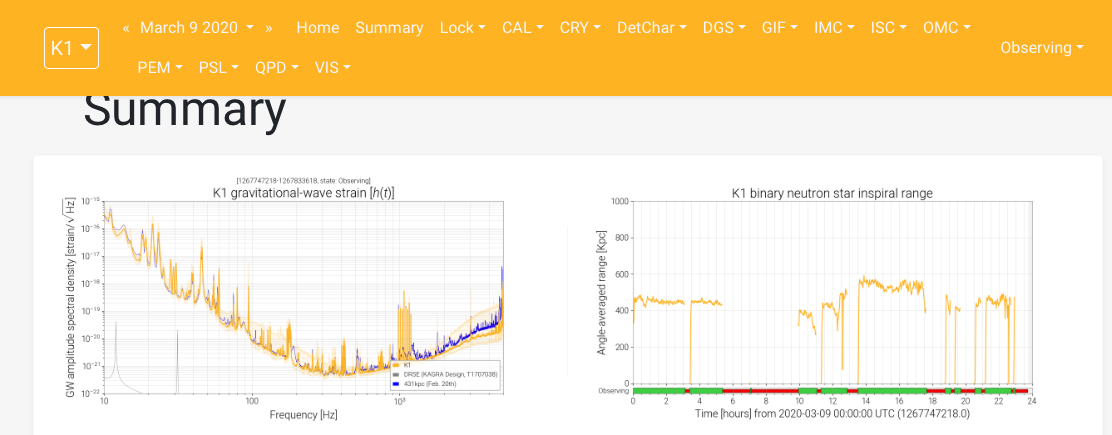
\includegraphics[width=0.48\textwidth]{astrodiv/gw/detc/png/det_summary.png}
\end{center}
\end{figure}

%!TEX root = ../../../2019main.tex
\vspace{10pt}
\subsubsection*{\bf Physical Environment Monitors}
\vspace{3pt}
\noindent {\sf [Spokesperson :\ Takaaki YOKOZAWA ]}

\vspace{3pt}
\noindent {\sf \small ICRR, The Univ.\ of Tokyo, Hida, Gifu 506-1205}

\vspace{3pt}

Because the amplitude of gravitational waves(GWs) are very small, 
we must take care everything which can be a noise source.
One of the major noise sources is environmental disturbance through earthquakes, 
effects from magnetic and acoustic fields, temperature and so on.
To investigate the effect from the environmental noise, 
we installed various types of the monitors, which are called as
physical environmental monitors (PEMs).
Also, because KAGRA interferometer was developed in the underground environment and 
operated with cryogenic temperature (20K).
Those environment and technique is essential to the next generation
GW interferometer. 
So the understanding of the KAGRA interferometer environment is  key technology.

Six seismometers were installed to evaluate the ground motion in the
underground environment and those seismometer were also used for the suspension 
control to reduce the mirror motion.
the accelerometers and microphones were also installed to monitor the optical tables.
Such auxiliary optics on the optical tables were used for many purpose, such as 
laser source stabilization, mode matching, sensing for the interferometer control and 
controls of the photon calibrator.
Those PEMs were used for evaluating not only the stationary interferometer noise but also
narrow band frequency noise and transient noise identification.

The temperature monitor is also important for keep the suspensions healthy.
If the temperature changed 1 degree, the height of the mirror motion was changed and 
it became difficult to keep the interferometer condition.
For monitoring the temperature, we installed total 77 thermometer, which can monitor both
temperature and humidity and made the web site to monitor the temperature drift.

Finally, to evaluate the effect from the environments, we established the system of the 
environmental injection, such as acoustic injection and magnetic injection system.
By performing the acoustic injection, we turned out that the peaks of the 160, 280 and 
360 Hz came from the acoustic environmental noise.

%\input{astrodiv/gw/mir/mir.tex}
%!TEX root = ../../../2019main.tex

\vspace{10pt}
\subsubsection*{\bf Commissioning}
\vspace{3pt}
\noindent {\sf [Spokesperson :\ Osamu MIYAKAWA]}

\vspace{3pt}
\noindent {\sf \small ICRR, The Univ.\ of Tokyo, Hida, Gifu 506-1205}

\vspace{3pt}

For KAGRA, it is not an exaggeration to say that the fiscal year of 2019 has been a year of commissioning. By FY2018, almost all of the subsystems had been installed and in FY2019 we targeted to operate as a whole interferometer. We had several engineering runs with the Michelson interferometer, operating in a single arm cavity, and finally carried it through to observation. It is a remarkable result that we were able to achieve the minimum target sensitivity of 1 MPc. This led to a joint observation with GEO.

In this process, one major problem was exposed: the presence of birefringence in the Sapphire mirror, which was thought to reduce the returning light from the interferometer.  This can be a direct problem for sensitivity since the target power-recycling gain cannot be achieved. It was then found that the modal healing effect of the arm cavity relieved this problem and that sufficient power recycling gain could be obtained. However, the sidebands would still be lost due to the birefringence, so we should consider making the mirror again in order to achieve the final sensitivity.

\begin{figure*}[htbp]
\begin{center}
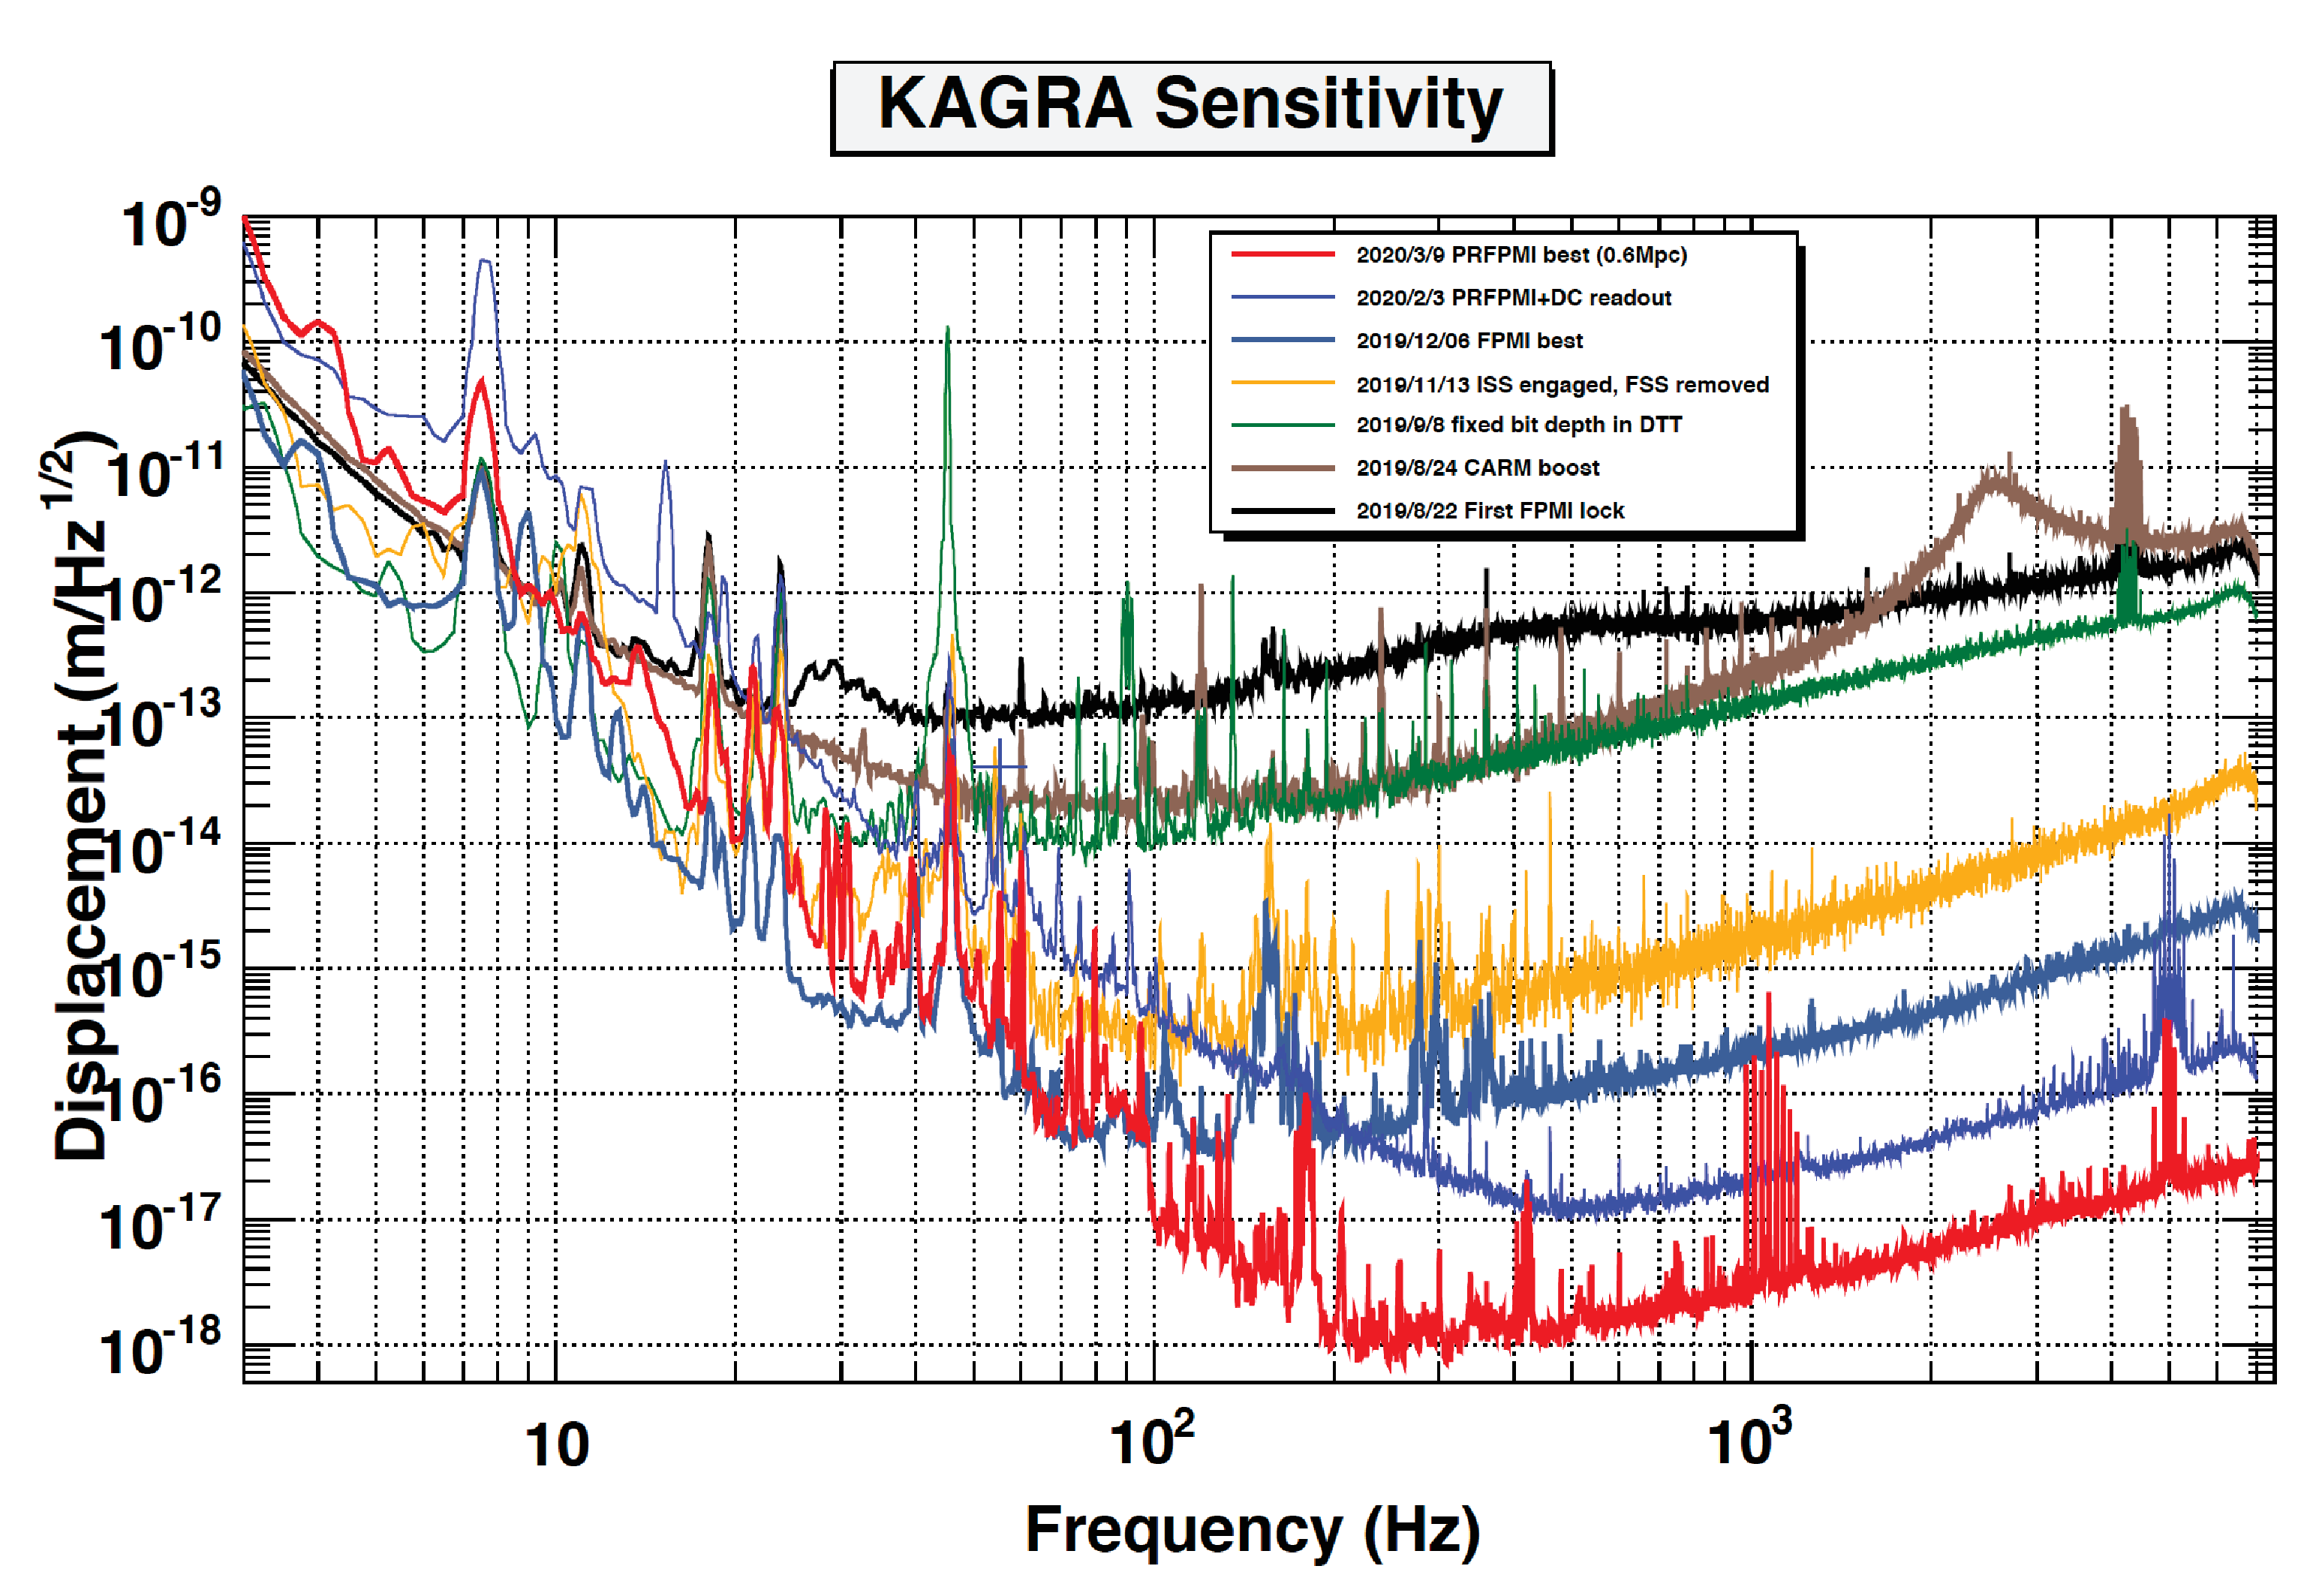
\includegraphics[width=14cm]{astrodiv/gw/commissioning/sens_improve.eps}
\caption{Improvement of the KAGRA sensitivity in 6 months.}
\label{fig:sens_improve}
\end{center}
\end{figure*}


The Fig.\ref{fig:sens_improve} shows the improvement in sensitivity over a period of about six months. We successfully achieved the first FPMI operation in late August, with both 3\,km arms  storing light into the arm cavities, and the first sensitivity was measured. At this point, it was found that 4-5 orders of magnitude were necessary to reach the minimum target sensitivity, and we realized that noise-hunting was the most important task for commissioning. We improved the sensitivity initially by resolving a few minor problems. When the sensitivity improvement was a bit slow, the introduction of the ISS (Intensity Stabilization Servo) improved by one order, and the removal of the FSS (Frequency Stabilization Servo) improved by another order of magnitude, total improvement in sensitivity by two orders of magnitude was not insignificant at that time. We continued to try to improve the sensitivity, but since we were using only 10\% of the transmitted light of the power recycling mirror, it was difficult to increase the laser power in the interferometer further, which limited the sensitivity at high frequencies.

In January, the PRFPMI which aimed to increase laser power in the interferometer was successfully operated. The laser power could be increased by a factor of 100 compared to the FPMI state. Although there were some concerns about the noise in the control systems, it was found that they did not limit the final sensitivity of the PRFPMI for the observations in 2019, and the operation of PRFPMI was fine. However, we believe that we need to move to DRFPMI to realize the final sensitivity as designed.

The following February we successfully established the OMC (output mode cleaner) in operation. This OMC allowed us to measure the sensitivity of the interferometer using DC power. This is called as a DC readout method that was designed as an final method without using RF sideband signals. The first sensitivity of the DC readout was 40\,kpc, which was almost the same as the highest sensitivity of FPMI, and we aimed to improve the sensitivity further. From this point, we improved the sensitivity by one more order of magnitude, and when the sensitivity was about 400\,kpc, we started the first observation for two weeks. During the observation, the sensitivity fluctuated several times due to uncertainties of calibration. This issue is still under investigation, and further verification is necessary. Finally, we achieved the minimum target sensitivity of 1\,Mpc, and this led to the second round of observations in April.

Through this commissioning, it was found that both sensitivity and stability are highly dependent on the alignment of mirrors. The angular control of the mirror has been successfully introduced in some degrees of freedom. In order to achieve the final sensitivity, it is necessary to introduce the angular control for all the degrees of freedom. It was also exposed that weakness for climate change, such as micro seismic motion in the 0.1 Hz band existed. This needs to be resolved by improving the control system of the vibration isolation system.

There were various problems and issues during the commissioning process, and most of them were solved and the stable operation was achieved. Although, there are still some problems to be solved, but it is remarkable that we have established the 4-5 orders of magnitude improvement of the sensitivity in only 6\,months. In the future, we will update the vibration isolation system and try to achieve the final target sensitivity through further commissioning.




%!TEX root = ../../../2019main.tex
\vspace{10pt}
\subsubsection*{\bf Observation}
\vspace{3pt}
\noindent {\sf [Spokesperson :\ Shinji MIYOKI]}

\vspace{3pt}
\noindent {\sf \small ICRR, The Univ.\ of Tokyo, Hida, Gifu 506-1205}

\vspace{3pt}

After the commissioning as referred in the previous paragraph, KAGRA has finally started its GW observation from 25th February to March 7th with 250 kpc $\sim$ 500 kpc binary range sensitivity for GWs from BNS mergers. After that, another GW network observation with GEO600 gravitational wave telescope was done from 7th April to 21st April with about 500 kpc $\sim$ 800kpc sensitivity. Between these two observations, an additional commissioning was performed to enhance its sensitivity and stability as a telescope. Finally, KAGRA sensitivity reached around 1 Mpc that was one of criteria for KAGRA to join the GW observation network with Adv.LIGO, Adv.Virgo and GEO600. In order to participate in this international GW observation network with Adv.LIGO, Adv.Virgo and GEO600, not only the sensitivity around 1 Mpc binary range, but also many requested criteria were cleared. They are (1) calibration of time domain strain sensitivity, h(t), and its uncertainty budget, (2) preparation of state vector information, (3) rapid response team formation, (4) low-latency KAGRA data transfer to CIT/Virgo, (5) collaboration general computing support, (6) data quality segment database preparation, (7) webpage for IFO status monitor and (8) high-latency data transfer between KAGRA and LV from the October 2019. The latter observation was regarded as ``O3GK'' that were performed according to the LVK MOA that was made in October in 2019. During O3GK, However, Adv.LIGO and Adv.Virgo were offline because of COVID-19 problems. Both observations had engineering runs for a week just before each observation for mainly calibration. Calibration was also done just after observations to evaluate the error range of KAGRA sensitivity. Each observation was operated in three shift system by one operator and one co-operator those were supported by expert members for operational emergency. The duty cycle for O3GK was 53.2\% in science mode and 58.8\% in locked mode. During the online state of both KAGRA and GEO600 during O3GK, an astronomical gamma-ray burst event named ``GRB200415A'' was reported. We are now analyzing our data on this event. 
%!TEX root = ../../../2019main.tex
\vspace{10pt}
\subsubsection*{\bf Data Analysis}
\vspace{3pt}
\noindent {\sf [Spokesperson :\ Hideyuki Tagoshi]}

\vspace{3pt}
\noindent {\sf \small ICRR, The Univ.\ of Tokyo, Kashiwa, Chiba, 277-8582}

\vspace{3pt}
There are variety of data related activities in KAGRA. 
The main data server of KAGRA is located at ICRR Kashiwa. It has a 2.5PiB data storage. 
All KAGRA data taken at Kamioka are packed into one file for every 32 seconds, 
and are transferred continuously to the main data server at Kashiwa. Beside this, low latency data transfer 
is also done by packing only main interferometer data into one file for every 1 seconds. 
For low latency data transfer, the latency of about 3 seconds is achieved from Kamioka to Kashiwa
(this time include the time necessary for calibration). 

KAGRA detector is producing several hundreds thousands of channels of data which record 
signals from various sensors, signals to control instruments, signals to monitor environment of the detector. 
Those data are used to check the status of detector and to improve the sensitivity. 
It is important to introduce convenient tools to visualize the data in order to accelerate the installation 
and commissioning works.  
Web based visualization tools are now being developed. Some of tools developed by LIGO group are also installed. 
These tools are also useful when gravitational wave signals are detected. 
In order to have a confidence of detection of gravitational wave signals, 
it is important to investigate environmental channels whether there are any noise sources which might 
produce data which are similar to real gravitational wave signals. 
These visualization tools can be used to check various  environmental channel data. 


In order to detect gravitational wave signals, several pipelines have been developed in KAGRA. 
Among them, a pipeline to search for gravitational waves from compact binary coalescences (CBC) 
are developed in KAGRA Algorithmic Library (KAGALI). KAGALI is a common data analysis library 
written mainly in C. The CBC pipeline have been used to analyze KAGRA data during iKAGRA operation. 
Improvement of the CBC pipeline are now ongoing in order to treat multiple detectors and 
to introduce the spin parameters in the waveform. These tasks will be continued in 2019. 
The improvement of the parameter estimation pipeline for CBC signals 
based on the Markov Chain Monte Carlo method was continued from the last year. 
This work is lead by Hyung Won Lee (Inje Univ). 

There are several efforts to introduce new data analysis methods in the analysis of gravitational wave data. 
Among them, the performance of Non-Harmonic Analysis (NHA) in visualizing the time-frequency behavior 
of the data was evaluated. NHA is a method to evaluate the spectrum of data 
by evaluating multiple instantaneous frequencies and amplitudes of data in a way which is different from 
discrete Fourier transform. We find that there are various advantage in NHA in visualizing CBC signals 
compared with the method of short time Fourier transform. We apply NHA to public data of 
LIGO-Virgo events, like GW150914, GW170817, and demonstrated the visualization of the signal 
on time-frequency plane. This work has been done in collaboration with the group of Shigeki Hirobayashi
(Univ. Toyama). 

~\\
\noindent
Ref.~~Kenta Yanagisawa , Dongbao Jia, Shigeki Hirobayashi, Nami Uchikata , Tatsuya Narikawa, Koh Ueno, Hirotaka Takahashi, Hideyuki Tagoshi, PTEP 2019 (2019) no.6, 063F01.

\begin{figure} [hbtp]
\begin{center}
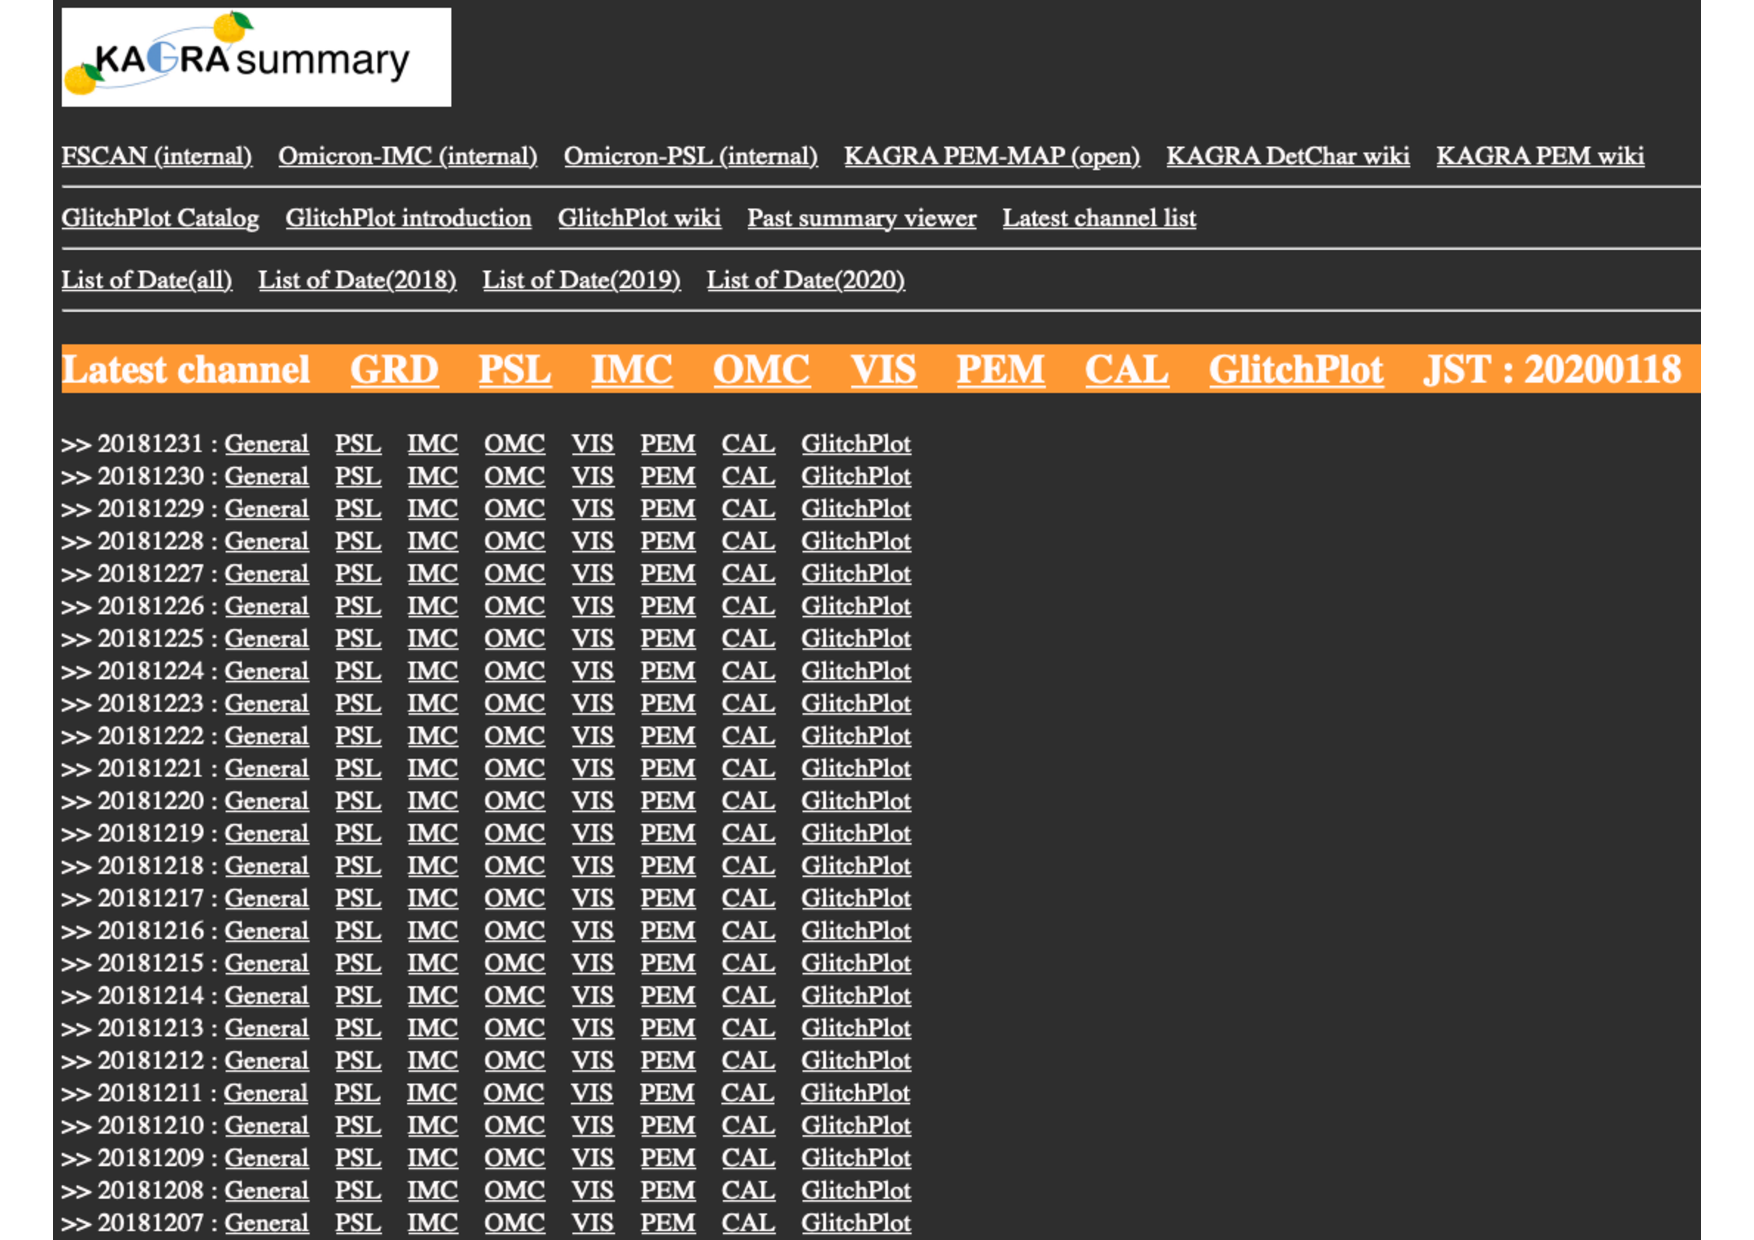
\includegraphics[width=8cm]{astrodiv/gw/das/fig/figdas.pdf}
\caption{\utsm \noindent{\narrower{Example of summary page}}}
\label{fig:KAGRA_DA_Sum}
\end{center}
\end{figure}





\vspace{12pt}
%%%%%%%%%%%%%%%%%%%%%%
  %
% sample project
%

%%%%%%%%%%%%%%%%%%%%%%%%%%%%%%%%%%%%%%%%%%%%%%%%%%%
% header 
%%%%%%%%%%%%%%%%%%%%%%%%%%%%%%%%%%%%%%%%%%%%%%%%%%%
\vspace{25pt}
\hrule
\section*{\bfsf Observational Cosmology Group} 
\vspace{12pt}
\hrule

\vspace{12pt}
\noindent
{\sf [Spokesperson : Yoshiaki Ono]}

\vspace{3pt}
\noindent
{\sf \small ICRR, The Univ. of Tokyo, Kashiwa, Chiba 277-8582}


\def\farcs{% 
 \mbox{% 
  \kern  0.13ex.% 
  \kern -0.95ex\raisebox{.9ex}{\scriptsize$\prime\prime$}% 
  \kern -0.1ex% 
 }% 
}

%\newcommand{\rqq}{\textquotedblright}
%\newcommand{\lqq}{\textquotedblleft}

%%%%%%%%%%%%%%%%%%%%%%%%%%%%%%%%%%%%%%%%%%%%%%%%%%%
% text 
%%%%%%%%%%%%%%%%%%%%%%%%%%%%%%%%%%%%%%%%%%%%%%%%%%%

\subsubsection*{\bi
SILVERRUSH. VIII. 
Spectroscopic Identifications of Early Large-scale Structures with Protoclusters 
over $200$ Mpc at $z\sim6$--$7$: 
Strong Associations of Dusty Star-forming Galaxies
{\rm \cite{harikane2019}}
}

\vspace{3pt}

\noindent
In collaboration with the members of 
\noindent
The University of Tokyo, 
National Astronomical Observatory of Japan, 
Aix Marseille University, 
Kitami Institute of Technology, 
California Institute of Technology, 
National Tsing Hua University, 
Osaka Sangyo University, 
Academia Sinica, 
University of California, Santa Barbara, 
Observatorio Nacional, 
Universidade de Sao Paulo, 
Durham University, 
RIKEN, 
Purple Mountain Observatory, 
Dalhousie University, 
Imperial College London, 
Seoul National University, 
Shanghai Jiao Tong University, 
Onomichi City University, 
Subaru Telescope, 
Nagoya University, 
Ehime University, 
and 
Cosmic Dawn Center. 

\vspace{10pt}

We have obtained three-dimensional maps of the universe 
in $\sim200\times200\times80$ comoving Mpc$^3$ (cMpc$^3$) volumes each at $z=5.7$ and $6.6$ 
based on a spectroscopic sample of 179 galaxies that achieves $\gtrsim80$\% completeness 
down to the Ly$\alpha$ luminosity of $\log(L_{\rm Ly\alpha}/[\mathrm{erg\ s^{-1}}])=43.0$, 
based on our Keck and Gemini observations and the literature 
(Figure \ref{cos:Harikane2019_Fig3}).
The maps reveal filamentary large-scale structures and two remarkable overdensities 
made out of at least 44 and 12 galaxies at $z=5.692$ (z57OD) and $z=6.585$ (z66OD), respectively, 
making z66OD the most distant overdensity spectroscopically confirmed to date, 
with $>10$ spectroscopically confirmed galaxies.
We compare spatial distributions of submillimeter galaxies at $z\simeq 4-6$ 
with our $z=5.7$ galaxies forming the large-scale structures, 
and detect a $99.97\%$ signal of cross-correlation, 
indicative of a clear coincidence of dusty star-forming galaxy and dust-unobscured galaxy formation 
at this early epoch.
The galaxies in z57OD and z66OD are actively forming stars with star-formation rates (SFRs) 
$\gtrsim5$ times higher than the main sequence, 
and particularly the SFR density (SFRD) in z57OD is 10 times higher than the cosmic average 
at the redshift (a.k.a. the Madau-Lilly plot).
Comparisons with numerical simulations suggest that 
z57OD and z66OD are protoclusters that are progenitors of the present-day clusters 
with halo masses of $\sim10^{14} M_\odot$.


%%%%%%%%%%%%%%%%%
% bibliography 
%%%%%%%%%%%%%%%%%

\begin{thebibliography}{9}
\bibitem[1]{harikane2019} 
Harikane, Y., Ouchi, M., Ono, Y., Fujimoto, S., Donevski, D., Shibuya, T., Faisst, A. L., Goto, T., Hatsukade, B., Kashikawa, N., Kohno, K., Hashimoto, T., Higuchi, R., Inoue, A. K., Lin, Y.-T., Martin, C. L., Overzier, R., Smail, I., Toshikawa, J., Umehata, H., Ao, Y., Chapman, S., Clements, D. L., Im, M., Jing, Y., Kawaguchi, T., Lee, C.-H., Lee, M. M., Lin, L., Matsuoka, Y., Marinello, M., Nagao, T., Onodera, M., Toft, S., Wang, W.-H. 
\ 2019, 
The Astrophysical Journal, 883, 142 
\end{thebibliography}


%--------------------------------------------------------------------------
\begin{figure}
\begin{center}
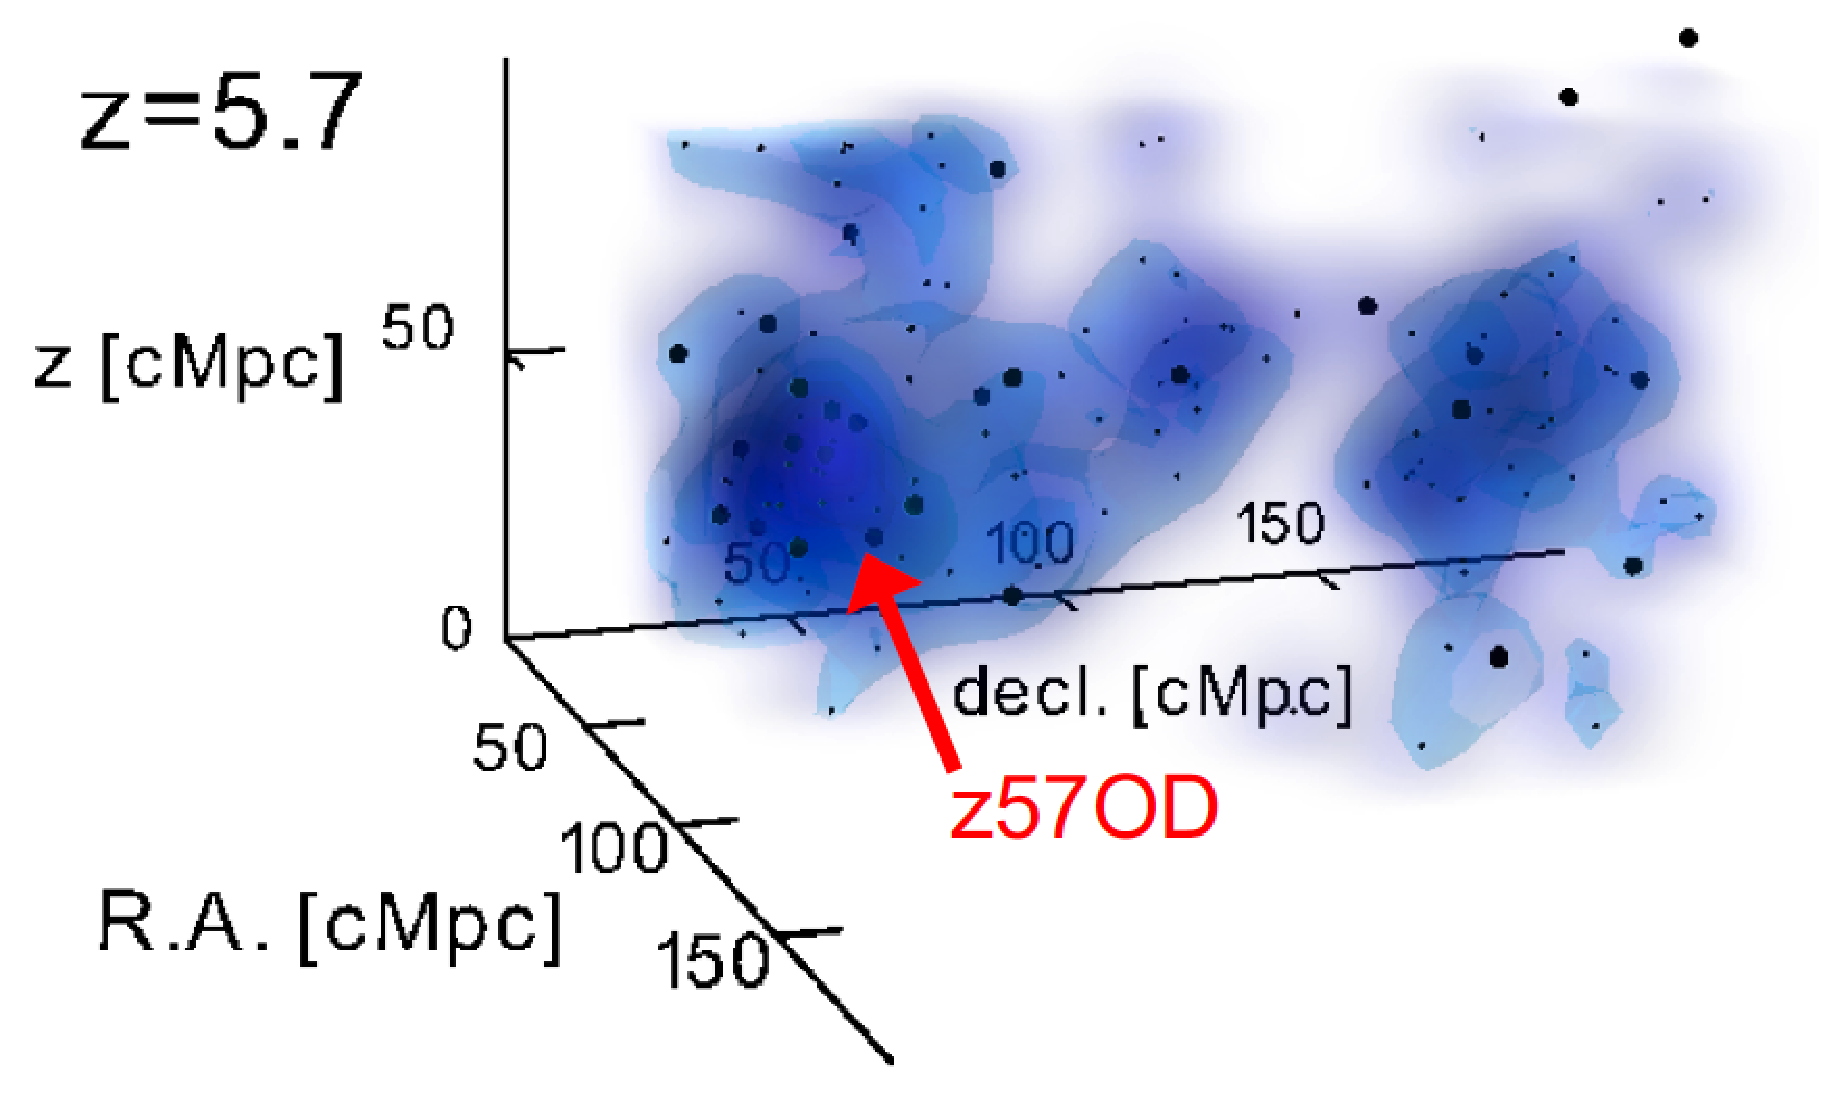
\includegraphics[height=4.7cm]{astrodiv/cos/Harikane2019_Fig3a.eps} 
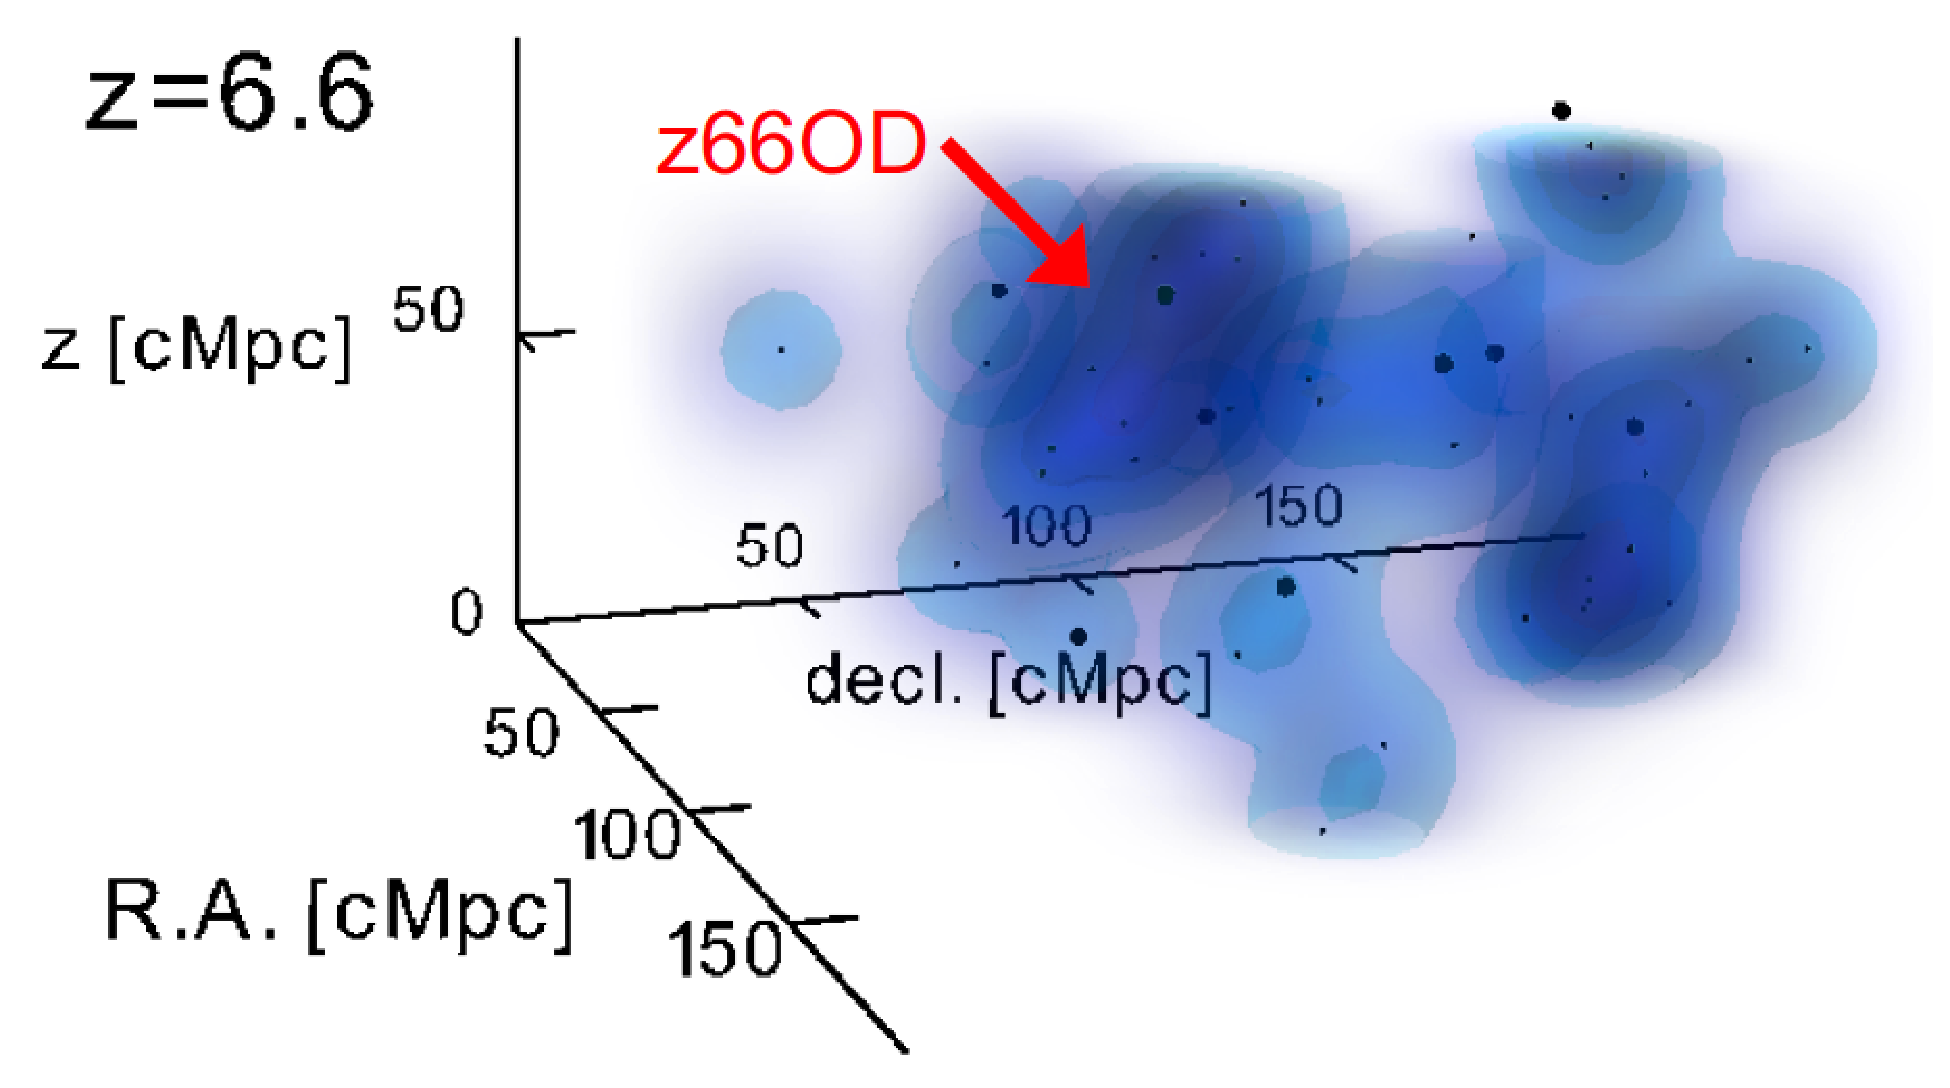
\includegraphics[height=4.7cm]{astrodiv/cos/Harikane2019_Fig3b.eps} 
\end{center}
\vspace{-5mm}
\caption{
3D overdensity maps of Ly$\alpha$ emitters (LAEs) at $z=5.7$ (top) and $z=6.6$ (bottom).
The black dots show the positions of the LAEs.
The large dots are LAEs brighter than $L_\mathrm{Ly\alpha}>10^{43}$ erg s$^{-1}$.
Higher density regions are indicated by the bluer colors, 
smoothed with a Gaussian kernel of $\sigma=10$ cMpc ($15$ cMpc) at $z=5.7$ ($z=6.6$).
}
\label{cos:Harikane2019_Fig3}
\end{figure}
%--------------------------------------------------------------------------






%%%%%%%%%%%%%%%%%%%%%%%%%%%%%%%%%%%%%%%%%%%%%%%%%%%
% text 
%%%%%%%%%%%%%%%%%%%%%%%%%%%%%%%%%%%%%%%%%%%%%%%%%%%

\subsubsection*{\bi
Fast Outflows Identified in Early Star-forming Galaxies at $z = 5$--$6$
{\rm \cite{sugahara2019}}
}

\vspace{3pt}

\noindent
In collaboration with the members of
\noindent
The University of Tokyo, 
National Astronomical Observatory of Japan, 
The University of Lyon, 
and 
Leiden Observatory. 

\vspace{10pt}

We present velocities of galactic outflows in seven star-forming galaxies at $z=5$--$6$ 
with stellar masses of $M_\ast \sim10^{10.1} M_\odot$. 
Although it is challenging to observationally determine the outflow velocities, 
we overcome this by using 
Atacama Large Millimeter/submillimeter Array (ALMA)
%ALMA 
[{\sc Cii}]158 $\mu$m emission lines for systemic velocities 
and deep Keck spectra with metal absorption lines for velocity profiles available to date. 
We construct a composite Keck spectrum of the galaxies at $z=5$--$6$ 
with the [{\sc Cii}]-systemic velocities, 
and fit outflow-line profiles to the Si{\sc ii}$\lambda1260$, C{\sc ii}$\lambda1335$, 
and Si{\sc iv}$\lambda\lambda1394,1403$ absorption lines in the composite spectrum. 
We measure the maximum (90\%) and central outflow velocities to be 
$v_{\rm max} = 700^{+180}_{-110}$ km s$^{-1}$ 
and $v_{\rm out} = 400^{+100}_{-150}$ km s$^{-1}$ on average, respectively, 
showing no significant differences between the outflow velocities 
derived with the low- to high-ionization absorption lines. 
For $M_\ast \sim10^{10.1} M_\odot$, 
we find that the $v_{\rm max}$ value of our $z=5$--$6$ galaxies is 3 times higher 
than those of $z\sim0$ galaxies and comparable to $z\sim2$ galaxies. 
Estimating the halo circular velocity $v_{\rm cir}$ from the stellar masses and the abundance matching results, 
we investigate a $v_{\rm max}$--$v_{\rm cir}$ relation (Figure \ref{cos:Sugahara2019_fig3}). 
Interestingly, $v_{\rm max}$ for galaxies with $M_\ast = 10^{10.0-10.8} M_\odot$ shows 
a clear positive correlation with $v_{\rm cir}$ and/or the galaxy star formation rate over $z=0$--$6$ 
with a small scatter of $\simeq \pm 0.1$ dex, 
which is in good agreement with theoretical predictions. 
This positive correlation suggests that the outflow velocity is physically related to the halo circular velocity, 
and that the redshift evolution of $v_{\rm max}$ at fixed $M_\ast$ 
is explained by the increase in $v_{\rm cir}$ toward high redshift.


%%%%%%%%%%%%%%%%%
% bibliography 
%%%%%%%%%%%%%%%%%

\begin{thebibliography}{9}
\bibitem[2]{sugahara2019} 
 Sugahara, Y., Ouchi, M., Harikane, Y., Bouch\'e, N., Mitchell, P. D., Blaizot, J. 
 \ 2019, 
The Astrophysical Journal, 886, 29 
\end{thebibliography}


%--------------------------------------------------------------------------
\begin{figure}
\begin{center}
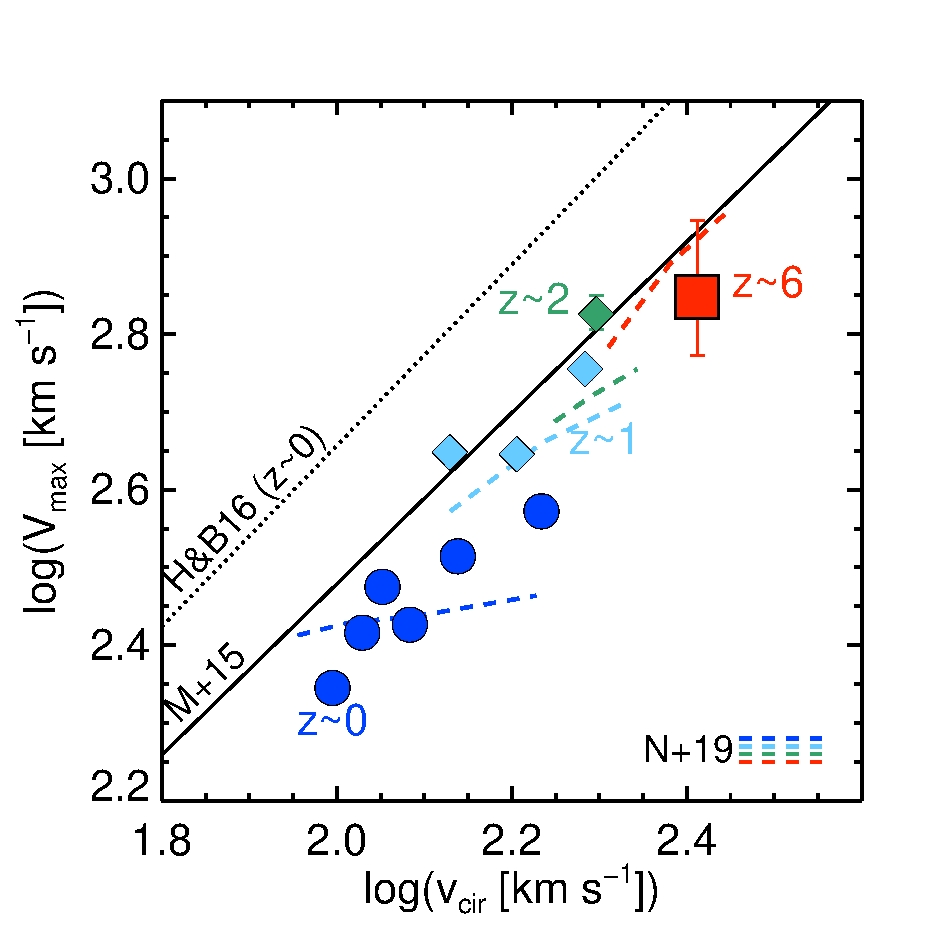
\includegraphics[width=8.5cm]{astrodiv/cos/Sugahara2019_Fig3.eps} 
\end{center}
\vspace{-5mm}
\caption{
$v_{\rm max}$ as a function of the circular velocity $v_{\rm cir}$ that are converted from the stellar mass. 
%The symbols are the same as in Figure \ref{fig:res1}. 
The filled red square indicates our results at $z=5$--$6$ 
measured with the simultaneous fitting of the Si{\sc ii} and {\sc Cii} lines. 
The data points at $z\sim0$ (blue) and $z\sim1$ (cyan) are 
taken from our previous work. 
%presented by Sugahara et al. (2017). 
The data point at $z\sim2$ is 
derived from the composite spectrum in our previous work, 
but re-calculated in the manner of this work
%The $v_{\rm max}$ value at $z\sim2$ (green) is 
%derived from the composite spectrum in Sugahara et al. (2017), but re-calculated in the manner of this work.
%
The solid, dashed, and dotted lines are obtained in the literature. 
The solid black line and colored dashed lines represent a theoretical relation at $z=0.5$--$4$ 
predicted by the FIRE simulations 
(the flux-weighted average 90th percentile velocity) 
%\citep[the flux-weighted average 90th percentile velocity;][]{Muratov:2015} 
and relations at $z=0$ (blue), $1$ (cyan), $2$ (green), and $6$ (red) 
predicted by the IllustrisTNG simulation 
(90th percentile velocity), 
%\citep[90th percentile velocity;][]{Nelson.D:2019a}, 
respectively. 
The dotted line indicates a relation of extreme-starburst galaxies $z\sim0$. 
%\citet{Heckman:2016}.
}
\label{cos:Sugahara2019_fig3}
\end{figure}
%--------------------------------------------------------------------------









%%%%%%%%%%%%%%%%%%%%%%%%%%%%%%%%%%%%%%%%%%%%%%%%%%%
% text 
%%%%%%%%%%%%%%%%%%%%%%%%%%%%%%%%%%%%%%%%%%%%%%%%%%%

\subsubsection*{\bi
First Identification of $10$ kpc [{\sc Cii}] $158\mu$m Halos around Star-forming Galaxies at $z = 5$--$7$ 
{\rm \cite{fujimoto2019}}
}

\vspace{3pt}

\noindent
In collaboration with the members of
\noindent
The University of Tokyo, 
National Astronomical Observatory of Japan, 
Waseda University, 
Scuola Normale Superiore, 
Centro Fermi, 
European Southern Observatory, 
University of Edinburgh, 
Osaka University, 
University of Tsukuba, 
and 
University of Nevada. 

\vspace{10pt}

We report the discovery of 10 kpc {\sc [Cii]} 158$\mu$m halos 
surrounding star-forming galaxies in the early Universe. 
We choose deep ALMA data of 18 galaxies, 
each with a star-formation rate of $\simeq 10$--$70\,M_\odot$ 
with no signature of 
%AGN
active galactic nucleus (AGN) 
whose {\sc [Cii]} lines are individually detected at $z=5.153$--$7.142$,
and we conduct stacking of the {\sc [Cii]} lines and dust continuum 
in the $uv$-visibility plane. 
The radial profiles of the surface brightnesses show a 10 kpc scale {\sc [Cii]} halo 
at the 9.2$\sigma$ level, significantly more extended than the 
\textit{Hubble Space Telescope} (HST) stellar continuum data
by a factor of $\sim5$ on the exponential-profile basis, as well as the dust continuum 
(Figure \ref{cos:fujimoto2019_fig11}).
We compare the radial profiles of {\sc [Cii]} and Ly$\alpha$ halos
universally found in star-forming galaxies at this epoch, 
and find that the scale lengths agree within $1\sigma$ level.
While two independent hydrodynamic zoom-in simulations match the dust and stellar continuum properties, 
the simulations cannot reproduce the extended {\sc [Cii]} line emission.
The existence of the extended {\sc [Cii]} halo is evidence of outflow remnants in the early galaxies 
and suggests that the outflows may be dominated by cold-mode outflows expelling the neutral gas. 

%%%%%%%%%%%%%%%%%
% bibliography 
%%%%%%%%%%%%%%%%%

\begin{thebibliography}{9}
\bibitem[3]{fujimoto2019} 
Fujimoto, S., Ouchi, M., Ferrara, A., Pallottini, A., Ivison, R. J., Behrens, C., Gallerani, S., Arata, S., Yajima, H., Nagamine, K. 
\ 2019, 
The Astrophysical Journal, 887, 107 
\end{thebibliography}


%--------------------------------------------------------------------------
\begin{figure*}
\begin{center}
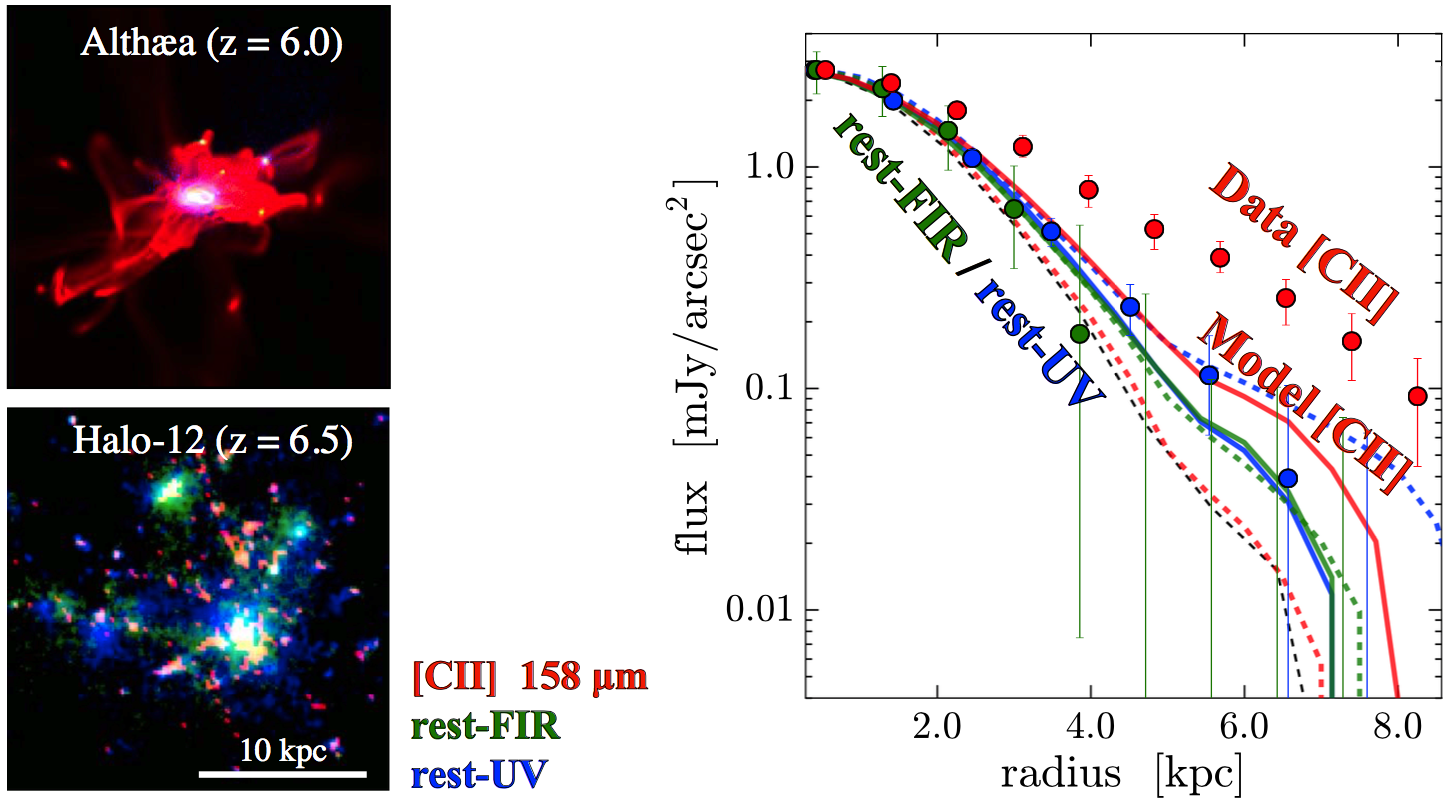
\includegraphics[width=16cm]{astrodiv/cos/Fujimoto2019_Fig11.eps} 
\end{center}
\vspace{-5mm}
\caption{
{\it \bf Left:} 
$4''\times4''$ fake-color image for Alth$\ae$a at $z=6.0$ (top) and Halo-12 (bottom) in the zoom-in simulations 
(red: {\sc [Cii]} line, green: rest-frame 
far-infrared (FIR)  
%FIR 
continuum, blue: rest-frame UV continuum). 
{\it \bf Right:} 
radial surface brightness profiles of the {\sc [Cii]} line (red curve), rest-frame FIR (green curve), and UV (blue curve) continuum emission estimated in the zoom-in simulations via a stacking procedure. 
The solid and dashed color lines represent the Alth$\ae$a and Halo-12 results, respectively.  
The black dashed curve denotes the ALMA synthesized beam. 
The circles indicate the ALMA-HST stacking results, whose colors are assigned in the same manner as the left panel.  
}
\label{cos:fujimoto2019_fig11}
\end{figure*}
%--------------------------------------------------------------------------






%%%%%%%%%%%%%%%%%%%%%%%%%%%%%%%%%%%%%%%%%%%%%%%%%%%
% text 
%%%%%%%%%%%%%%%%%%%%%%%%%%%%%%%%%%%%%%%%%%%%%%%%%%%

\subsubsection*{\bi
Balmer Break Galaxy Candidates at $z\sim6$: 
A Potential View on the Star Formation Activity at $z \gtrsim 14$ 
{\rm \cite{mawatari2020}}
}

\vspace{3pt}

\noindent
In collaboration with the members of
\noindent
Osaka Sangyo University, 
Waseda University, 
National Astronomical Observatory of Japan, 
University of Tsukuba, 
The University of Tokyo, 
Ehime University, 
Japan Aerospace Exploration Agency, 
Tohoku University, 
California Institute of Technology, 
Academia Sinica, 
and 
The Open University of Japan. 

\vspace{10pt}

We search for galaxies with a strong Balmer break (Balmer Break Galaxies; BBGs) 
at $z \sim 6$ over a 0.41\,deg$^2$ effective area in the COSMOS field. 
Based on rich imaging data, including data obtained with the ALMA, 
%Atacama Large Millimeter/submillimeter Array (ALMA), 
three candidates are identified by their extremely red $K - [3.6]$ colors, 
as well as by non-detection in X-ray, optical, 
%far-infrared (FIR), 
FIR, 
and radio bands. 
The non-detection in the deep ALMA observations suggests that 
they are not dusty galaxies but BBGs at $z \sim 6$, 
although contamination from 
%active galactic nuclei (AGNs) 
AGNs 
at $z \sim 0$ cannot be completely ruled out for the moment.
Our spectral energy distribution (SED) analyses reveal that 
the BBG candidates at $z \sim 6$ have stellar masses of $\approx 5 \times 10^{10}\,M_{\odot}$ 
dominated by old stellar populations with ages of $\gtrsim 700$ Myr. 
Assuming that all the three candidates are real BBGs at $z \sim 6$, 
we estimate the stellar mass density (SMD) to be $2.4^{+2.3}_{-1.3} \times 10^{4}\,M_{\odot}$\,Mpc$^{-3}$ 
(Figure \ref{cos:Mawatari2020_fig13}). 
This is consistent with an extrapolation from the lower-redshift measurements. 
The onset of star formation in the three BBG candidates is expected to be several hundred million years 
before the observed epoch of $z \sim 6$. 
We estimate the 
%star-formation rate density (SFRD) 
SFRD 
contributed by progenitors of the BBGs 
to be ($2.4$--$12) \times 10^{-5}\,M_{\odot}$\,yr$^{-1}\,$Mpc$^{-3}$ at $z > 14$ (99.7\% confidence range). 
Our result suggests a smooth evolution of the SFRD beyond $z = 8$. 

%%%%%%%%%%%%%%%%%
% bibliography 
%%%%%%%%%%%%%%%%%

\begin{thebibliography}{9}
\bibitem[4]{mawatari2020} 
Mawatari, K., Inoue, A. K., Hashimoto, T., Silverman, J., Kajisawa, M., Yamanaka, S., Yamada, T., Davidzon, I., Capak, P., Lin, L., Hsieh, B.-C., Taniguchi, Y., Tanaka, M., Ono, Y., Harikane, Y., Sugahara, Y., Fujimoto, S., Nagao, T. 
\ 2020, 
The Astrophysical Journal, 889, 137 
\end{thebibliography}



%--------------------------------------------------------------------------
\begin{figure}
\begin{center}
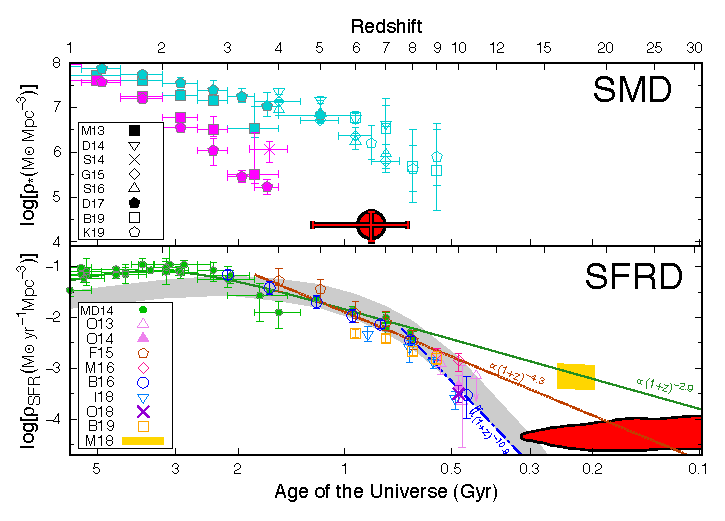
\includegraphics[width=8.5cm]{astrodiv/cos/Mawatari2020_Fig13.eps} 
\end{center}
\vspace{-5mm}
\caption{
Evolution of the SMD (top) and the SFRD (bottom) along the cosmic history (see top axis for the corresponding redshift). 
For these plots, we assume all the three BBG candidates without ALMA detection to be real passive galaxies at $z \sim 6$. 
In the top panel, the SMD of our BBG sample at $z \sim 6$ (red circle) is shown 
in conjunction with those of star-forming (cyan symbols) and passive (magenta symbols) galaxies at lower redshifts 
from the literature. 
%(M13: \citealt{Muzzin+13c}, D14: \citealt{Duncan+14}, S14: \citealt{Straatman+14}, G15: \citealt{Grazian+15}, S16: \citealt{Song+16}, D17: \citealt{Davidzon+17}, B19: \citealt{Bhatawdekar+19}, and K19: \citealt{Kikuchihara+19}). 
The vertical error bar associated with our BBG data corresponds to a $1\,\sigma$ uncertainty 
propagated from the Poisson error 
%\citep{Gehrels86} 
for the BBG number and the SED fitting uncertainty for the stellar mass. 
The horizontal error bar shows the redshift range expected from our BBG color selection. 
In the bottom panel, the red shaded region corresponds to the SFRD 
expected from the progenitors of the $z \sim 6$ BBGs at a $99.7$\,\% confidence level ($3\,\sigma$). 
The SFRD measurements at $z \lesssim 10$ are collected from the literature 
%(MD14: \citealt{Madau+14}, O13: \citealt{Oesch+13b}, O14: \citealt{Oesch+14}, F15: \citealt{Finkelstein+15a}, M16: \citealt{McLeod+16}, B16: \citealt{Bouwens+16c}, I18: \citealt{Ishigaki+18}, O18: \citealt{Oesch+18a}, and B19: \citealt{Bhatawdekar+19}). 
All of them at $4 \lesssim z \lesssim 10$ are estimated by integrating the UV 
luminosity functions 
%LFs 
down to $M_{\rm UV} = -17$\,mag. 
The SFRD estimated at $z \sim 17$ from an observed global 21\,cm absorption trough 
%(M18: \citealt{Madau18}, \citealt{Bowman+18}) 
is also shown in yellow. 
The functional fit to the MD14 data, which is proportional to $(1 + z)^{-2.9}$ at high-$z$,  
%\citep{Madau+14}, 
is superposed by the solid line. 
Two other power-law functions supporting an accelerated evolution at $z \gtrsim 8$ 
($\rho_{\rm SFR} \propto (1+z)^{-10.9}$)
%; \citealt{Oesch+14}) 
and a smooth evolution from lower redshift ($\rho_{\rm SFR} \propto (1+z)^{-4.3}$)
%; \citealt{Finkelstein+15a}) 
are shown by dotted-dashed and dotted lines, respectively. 
The SFRD derived assuming a universal relation among the halo mass, SFR, and dark matter accretion rate 
%\citep{Harikane+18a} 
is also superposed by the gray shade in its $1\,\sigma$ uncertainty. 
All of the SMD and SFRD measurements from the literature are corrected for the stellar IMF 
and the cosmological model to match those in this work. 
}
\label{cos:Mawatari2020_fig13}
\end{figure}
%--------------------------------------------------------------------------







%%%%%%%%%%%%%%%%%%%%%%%%%%%%%%%%%%%%%%%%%%%%%%%%%%%
% text 
%%%%%%%%%%%%%%%%%%%%%%%%%%%%%%%%%%%%%%%%%%%%%%%%%%%

\subsubsection*{\bi
CHORUS. III. Photometric and Spectroscopic Properties of Ly$\alpha$ Blobs at $z = 4.9$--$7.0$
{\rm \cite{zhang2020}}
}

\vspace{3pt}

\noindent
In collaboration with the members of
\noindent
The University of Tokyo, 
Kitami Institute of Technology, 
National Astronomical Observatory of Japan, 
Osaka Sangyo University, 
Waseda University, 
The Observatories of the Carnegie Institution for Science, 
University of Tsukuba, 
Osaka University, 
The Graduate University for Advanced Studies, 
Kure College, 
Observatoire de Geneve, 
Ehime University, 
and 
The Open University of Japan. 

\vspace{10pt}

We report the Subaru Hyper Suprime-Cam (HSC) discovery of two Ly$\alpha$ blobs (LABs), 
dubbed z70-1 and z49-1 at $z=6.965$ and $z=4.888$ respectively, 
that are Ly$\alpha$ emitters with a bright ($\log L_{\rm Ly\alpha}/{\rm [erg\ s^{-1}]}>43.4$) 
and spatially-extended Ly$\alpha$ emission, 
and present the photometric and spectroscopic properties of a total of seven LABs: 
the two new LABs and five previously known LABs at $z=5.7$--$6.6$. 
The z70-1 LAB shows extended Ly$\alpha$ emission with a scale length of $1.4\pm 0.2$ kpc, 
about three times larger than the UV continuum emission, 
making z70-1 the most distant LAB identified to date. 
All of the seven LABs, except z49-1, exhibit no AGN signatures such as X-ray emission, 
{\sc Nv}$\lambda$1240 emission, or Ly$\alpha$ line broadening, 
while z49-1 has a strong {\sc Civ}$\lambda$1548 emission line 
indicating an AGN on the basis of the UV-line ratio diagnostics. 
We carefully model the point-spread functions of the HSC images 
and conduct two-component exponential profile fitting 
to the extended Ly$\alpha$ emission of the LABs. 
The Ly$\alpha$ scale lengths of the core (star-forming region) 
and halo components are $r_{\rm c}=0.6$--$1.2$ kpc and $r_{\rm h}=2.0$--$13.8$ kpc, respectively. 
The relations between the scale lengths and galaxy properties 
(Ly$\alpha$ luminosity $L_{\rm Ly\alpha}$, Ly$\alpha$ rest-frame equivalent width EW$_0$, 
and UV continuum magnitude $M_{\rm UV}$) of our LABs 
are similar to those of Ly$\alpha$ halos (LAHs) 
identified around star-forming galaxies 
found previously by VLT/MUSE at similar redshifts (Figure \ref{cos:Zhang2020_Fig12}), 
suggesting that our LABs are likely the bright version of high-$z$ LAHs. 
%The average $r_{\rm h}$ of the LABs falls on the extrapolation of the $r_{\rm h}$-Ly$\alpha$ luminosity relation of the Ly$\alpha$ halos around VLT/MUSE star-forming galaxies at the similar redshifts, suggesting that typical LABs at $z\gtrsim5$ are not special objects, but star-forming galaxies at the bright end.

%%%%%%%%%%%%%%%%%
% bibliography 
%%%%%%%%%%%%%%%%%

\begin{thebibliography}{9}
\bibitem[5]{zhang2020} 
Zhang, H., Ouchi, M., Itoh, R., Shibuya, T., Ono, Y., Harikane, Y., Inoue, A. K., Rauch, M., Kikuchihara, S., Nakajima, K., Yajima, H., Arata, S., Abe, M., Iwata, I., Kashikawa, N., Kawanomoto, S., Kikuta, S., Kobayashi, M., Kusakabe, H., Mawatari, K., Nagao, T., Shimasaku, K., Taniguchi, Y.
\ 2020, 
The Astrophysical Journal, 891, 177 
\end{thebibliography}


%--------------------------------------------------------------------------
\begin{figure}
\begin{center}
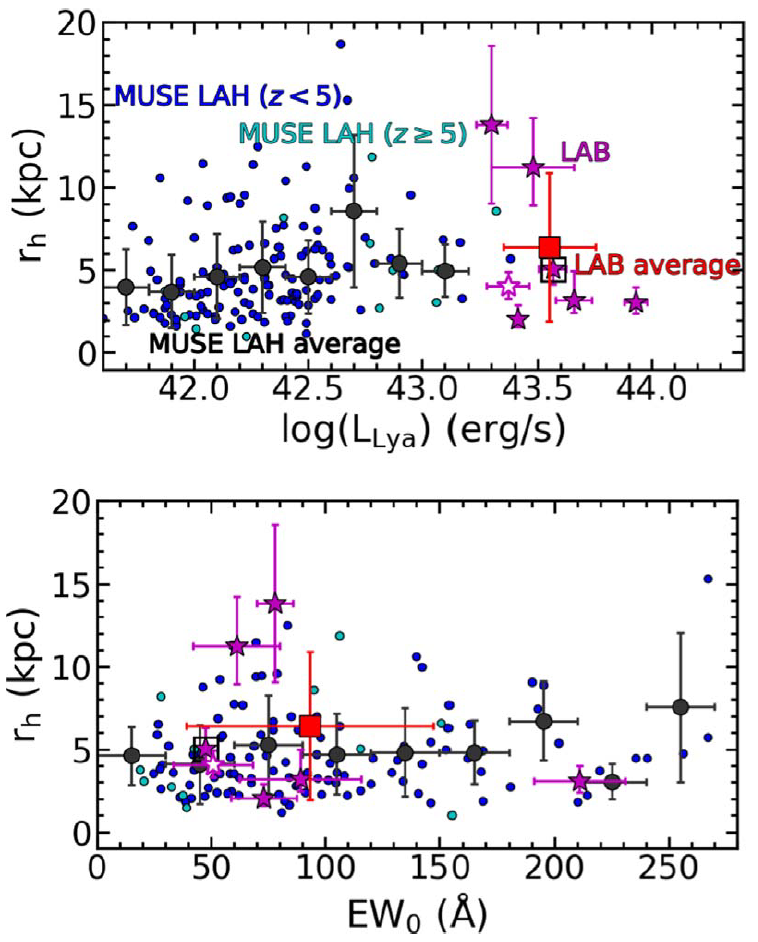
\includegraphics[width=8.5cm]{astrodiv/cos/Zhang2020_Fig12.eps} 
\end{center}
\vspace{-5mm}
\caption{
Halo scale length as a function of Ly$\alpha$ luminosity (top) and Ly$\alpha$ rest-frame equivalent width (bottom) 
of the seven LABs (stars) and LAHs (filled circles) from the literature. 
The empty star represents z57-2, which does not have a two-component fitting result. 
The red filled square shows the average value of our LABs, 
with error bars indicating the rms.  
The MUSE LAHs at $z<5$ and $z\geq5$ are the blue and cyan filled circles, respectively. 
The average values of the MUSE LAHs are shown as black filled circles. 
The black horizontal error bar indicates the bin size, 
while the black vertical error bar is the rms. 
%The solid lines represent the best-fit linear functions to the MUSE LAEs at $z=3-6$ (black) and $z=5-6$ (cyan), while the dashed lines are the extrapolations of the best-fit functions. It is clear that the average values of our LABs are consistent with the extrapolations of the best-fit functions of MUSE LAEs at $z=3-6$ and $z=5-6$. 
In the top panel, we slightly shift z49-1 (boxed star) along the horizontal axis by +0.03 to avoid overlaps.
}
\label{cos:Zhang2020_Fig12}
\end{figure}
%--------------------------------------------------------------------------



 
%  \input{astrodiv/theory/theory.tex} 
  %\color{black}
%\end{comment}

%%%%%%%%%%%%%%%%%%%%%%
% modify here (end)
%%%%%%%%%%%%%%%%%%%%%%

%\begin{comment}
    %\label{obs}
    %\input{obs/observa.tex} 
    \setcounter{figure}{0}
    \setcounter{table}{0}
    
    %\label{norikura}
%    \input{obs/Norikura/norikura.tex}
    \setcounter{figure}{0}
    \setcounter{table}{0}
    
    %\label{akeno}
%    \input{obs/Akeno/akeno_obs.tex}
    \setcounter{figure}{0}
    \setcounter{table}{0}
    
    %\label{kamioka}
%    \input{obs/kamobs/kamioka_obs.tex} 
    \setcounter{figure}{0}
    \setcounter{table}{0}
    
    %!TEX root = ../../2019main.tex
\onecolumn %% updated on 2017.7.19

\begin{center}
\hrule
\vspace{10pt}
{\bigsf KAGRA OBSERVATORY}
\label{kagra}
\vspace{10pt}
\hrule
\end{center}

\begin{multicols}{2}
KAGRA observatory is located in the Ikenoyama-mountain on the border
between Gifu and Toyama prefecture, about 35 km south of Toyama city in
Japan. The observatory was established in 2016 in order to operate Large
-scale Cryogenic Gravitational Wave Telescope (nicknamed “KAGRA”). KAGRA
itself has a L-shape tunnel facility, and it is located more than 200m
under Mt.Ikeno-yama. The corner station of the L-shape tunnel is
accessible through a 500-m horizontal access tunnel from Atotsu area.
The observatory has its own surface research buildings and rental space
in the community center of Hida city located about 5km away from the
Atotsu entrance of KAGRA.

KAGRA aims to observe several gravitational waves (GWs) per a year with
its designed sensitivity as one of observatories of the world GW
detection network including Advanced-LIGO, Advanced-Virgo and planned
LIGO-India. KAGRA project (formerly named LCGT) was partially approved
in 2010 as one of Leading-edge Research Infrastructure Program, and also
supported by Program for Promoting Large-scale Science Projects, Subsidy
for Facilities Expense and Grants-in-Aid for Scientific Research from
Ministry of Education, Culture, Sports, Science and Technology (MEXT).

In the KAGRA project, Institute for Cosmic Ray Research plays a role of a
host promoting institute, and National Astronomical Observatory in Japan
(NAOJ) and High Energy Accelerator Research Organization (KEK) are the
main support organizations, then more than 297 researchers in 85
institutes and universities in the world are collaborating for
construction and data analysis of KAGRA.

The tunnel excavation started in May 2012, and finished in March 2014.
After that, the basic laboratory environment was prepared until
September 2015. A Michelson interferometer with 3km arm (iKAGRA) was
demonstrated in March 2016, and the first engineering run was performed
until May 2016.  In 2019, all the interferometer components had been installed to complete 
the KAGRA Observatory that adopts a power recycled Fabry-Perot Michelson type interferometer 
with the resonant sideband extraction.
On February 25th, 2020, KAGRA started its first observation run. 
After performing the observation until April 2020, KAGRA will be upgraded and prepared
for the joint observation with LIGO and Virgo which is expected to start in the end of 2021.
\end{multicols} 

\medskip
\medskip
\medskip

\begin{figure}[htbp]
\begin{minipage}{0.5\textwidth}
\begin{center}
%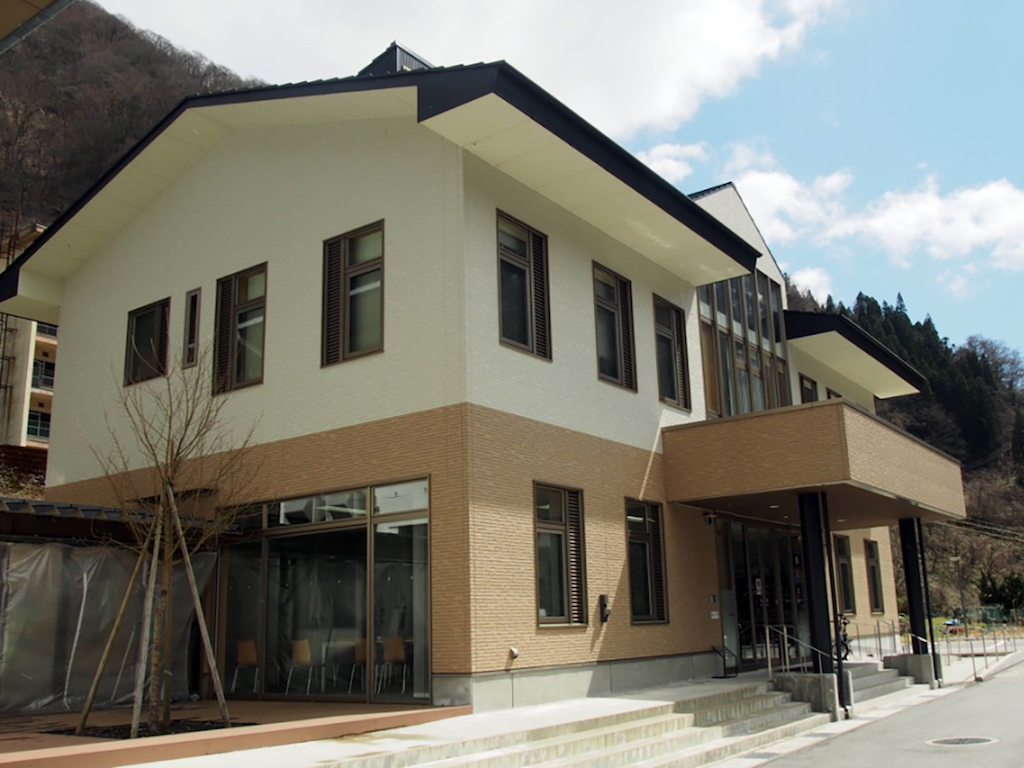
\includegraphics[width=0.8\textwidth]{./obs/kagra/building.jpg}
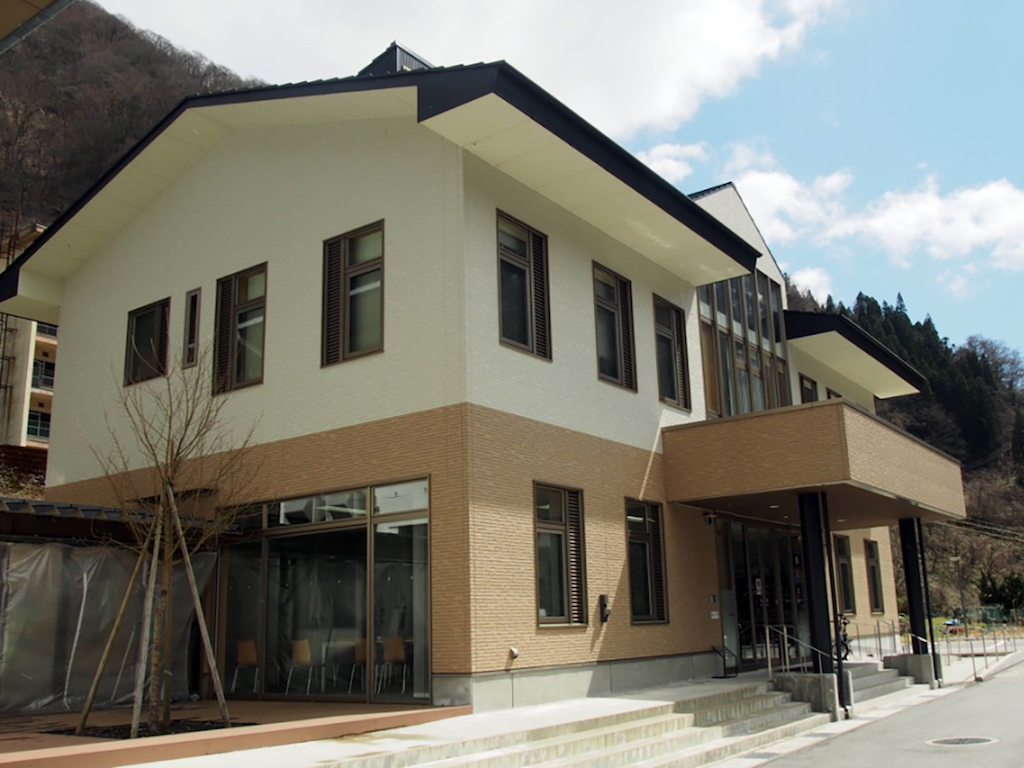
\includegraphics[height=6cm, bb=0 0 1024 768]{./obs/kagra/building.jpg}
\caption{Surface Research Building.}
\end{center}
\end{minipage}
%
\begin{minipage}{0.5\textwidth}
\begin{center}
%\includegraphics[width=0.8\textwidth]{./obs/kagra/entrance.jpg}
\includegraphics[height=6cm, bb=0 0 1089 722]{./obs/kagra/entrance.jpg}
\caption {Atotsu Entrance of KAGRA.}
\end{center}
\end{minipage}
\end{figure}



    \setcounter{figure}{0}
    \setcounter{table}{0}
    
    %\label{rccn}
%    \input{obs/rccn/rccn.tex}
    \setcounter{figure}{0}
    \setcounter{table}{0}
    
%    \input{app/Ap_contents.tex}
%    \input{app/Ap2018-2019.tex} 
%\end{comment}

\end{document}
